%%%%%%%%%%%%%%%%%%%%%%%%%%%%%%%%%%%%%%%%%%%%%%%%%%%
%% LaTeX book template                           %%
%% Author:  Amber Jain (http://amberj.devio.us/) %%
%% License: ISC license                          %%
%%%%%%%%%%%%%%%%%%%%%%%%%%%%%%%%%%%%%%%%%%%%%%%%%%%

\documentclass[a4paper,11pt]{book}
\usepackage[T1]{fontenc}
\usepackage[utf8]{inputenc}
\usepackage{lmodern}
%%%%%%%%%%%%%%%%%%%%%%%%%%%%%%%%%%%%%%%%%%%%%%%%%%%%%%%%%
% Source: http://en.wikibooks.org/wiki/LaTeX/Hyperlinks %
%%%%%%%%%%%%%%%%%%%%%%%%%%%%%%%%%%%%%%%%%%%%%%%%%%%%%%%%%
\usepackage{hyperref}
\usepackage{graphicx}
\usepackage{xcolor}
\usepackage{textcomp}
\usepackage[english]{babel}
\usepackage[a4paper,top=2cm,bottom=2cm,left=2cm,right=2cm]{geometry}
\usepackage{lscape}
\usepackage{caption}
\usepackage{amsmath}
\usepackage{listingsutf8}
\usepackage{listings}
\usepackage{wrapfig}
\usepackage{rotating}
\usepackage{epstopdf}

\usepackage[ruled]{algorithm2e}
\lstset{% general command to set parameter(s)
	basicstyle=\small, % print whole listing small
	numbers=left,
	keywordstyle=\color{black}\bfseries,
	% underlined bold black keywords
	identifierstyle=, % nothing happens
	stringstyle=\ttfamily} % typewriter type for strings

\lstset{language=Java} 
\captionsetup{tableposition=top,figureposition=bottom,font=small}
%%%%%%%%%%%%%%%%%%%%%%%%%%%%%%%%%%%%%%%%%%%%%%%%%%%%%%%%%%%%%%%%%%%%%%%%%%%%%%%%
% 'dedication' environment: To add a dedication paragraph at the start of book %
% Source: http://www.tug.org/pipermail/texhax/2010-June/015184.html            %
%%%%%%%%%%%%%%%%%%%%%%%%%%%%%%%%%%%%%%%%%%%%%%%%%%%%%%%%%%%%%%%%%%%%%%%%%%%%%%%%
\newenvironment{dedication}
{
   \cleardoublepage
   \thispagestyle{empty}
   \vspace*{\stretch{1}}
   \hfill\begin{minipage}[t]{0.66\textwidth}
   \raggedright
}
{
   \end{minipage}
   \vspace*{\stretch{3}}
   \clearpage
}

%%%%%%%%%%%%%%%%%%%%%%%%%%%%%%%%%%%%%%%%%%%%%%%%
% Chapter quote at the start of chapter        %
% Source: http://tex.stackexchange.com/a/53380 %
%%%%%%%%%%%%%%%%%%%%%%%%%%%%%%%%%%%%%%%%%%%%%%%%
\makeatletter
\renewcommand{\@chapapp}{}% Not necessary...
\newenvironment{chapquote}[2][2em]
  {\setlength{\@tempdima}{#1}%
   \def\chapquote@author{#2}%
   \parshape 1 \@tempdima \dimexpr\textwidth-2\@tempdima\relax%
   \itshape}
  {\par\normalfont\hfill--\ \chapquote@author\hspace*{\@tempdima}\par\bigskip}
\makeatother

%%%%%%%%%%%%%%%%%%%%%%%%%%%%%%%%%%%%%%%%%%%%%%%%%%%
% First page of book which contains 'stuff' like: %
%  - Book title, subtitle                         %
%  - Book author name                             %
%%%%%%%%%%%%%%%%%%%%%%%%%%%%%%%%%%%%%%%%%%%%%%%%%%%

% Book's title and subtitle
\title{\Huge \textbf{Gestione di un sistema di book-crossing:\\ \textit{\textbf{The WalkingBooks}}} \\ \huge \textit{\textbf{Documentazione progettuale}} \\ \bigskip \huge Progetto del corso di Informatica IIIB \\ \huge A.A. 2018/2019}
% Author
\author{\textsc{Paganessi Andrea} \\ \textsc{Piffari Michele} \\ \textsc{Villa Stefano}}


\begin{document}

\frontmatter
\maketitle

%%%%%%%%%%%%%%%%%%%%%%%%%%%%%%%%%%%%%%%%%%%%%%%%%%%%%%%%%%%%%%%%%%%%%%%%
% Auto-generated table of contents, list of figures and list of tables %
%%%%%%%%%%%%%%%%%%%%%%%%%%%%%%%%%%%%%%%%%%%%%%%%%%%%%%%%%%%%%%%%%%%%%%%%
\tableofcontents
\listoffigures
\listoftables

\mainmatter


\part{Iterazione 0}
\chapter{Requisiti e specifiche}
\section{Requisiti utente}
La startUp bergamasca Book Crossing UniBg desidera mettere a disposizione dei propri
utenti un'applicazione Android per poter gestire la libera condivisione di libri all'interno di una vasta community di utenti.

I libri della rete di BookCrossing che l'azienda punta a gestire si possono trovare
\begin{itemize}
	\item Casualmente (in stazione, su una panchina, in un locale o in un qualsiasi altro luogo): funzionalità \textit{"on the go"}
	\item Nella zona di scambio ufficiale (\textit{"OCZ UniBg"}: Official Crossing Zone UniBg)
\end{itemize}

Per il momento, l'unica OCZ gestita direttamente dalla startUp si trova all'interno dell'aula studio del campus di Ingegneria di Dalmine, la quale coincide anche con la sistemazione del server centrale che andrà a gestire i vari interscambi tra gli users.

La startUp richiede che, per usufruire dell'applicativo mobile, i clienti debbano registrarsi fornendo i propri dati quali
\begin{itemize}
	\item Nome
	\item Cognome
	\item Contatto di riferimento (opzionale)
	\begin{itemize}
		\item Numero telefonico
		\item Indirizzo mail
		\item Facebook
		\item ID Twitter
	\end{itemize}
	\item Categorie di libri preferite
	\item Zona di residenza
\end{itemize}

Una volta registratosi, l'utente può partecipare al programma di Book Crossing.

Secondo la politica del book sharing, per rendere disponibile alla comunità 
uno o più libri che non sono ancora presenti nel network stesso, 
serve
identificarli univocamente, per poterne così tracciare la storia, ovvero ciò 
che concerne il percorso seguito dal libro, le recensioni lasciate dagli utenti etc.

Prima di procedere con l'identificazione univoca del libro, l'utilizzatore deve inserire i dati 
del testo (o dei testi) che intende condividere con il resto della community: questo inserimento può avvenire
- In maniera "automatica" tramite scansione del codice ISBN
- In modalità "manuale", nel caso in cui, per esempio, non sia presente il barcode, fornendo i 
seguenti dati:
\begin{itemize}
	\item Titolo
	\item Autore
	\item Anno di pubblicazione/Edizione
	\item Categoria
\end{itemize}

A questo punto il sistema genererà un BCID di 10 caratteri, ovvero un \textit{Book Crossing ID} univoco, il
quale dovrà essere riportato sul testo dall'utente.


La vera e propria condivisione avviene nel momento in cui il volume/i viene rilasciato (azione che può avvenire in un secondo momento
rispetto alla fase di identificazione), il sistema dovrà acquisire i seguenti dati:
\begin{itemize}
	\item Luogo di rilascio (con estensione future per un'acquisizione automatica della posizione tramite GPS)
	\item Ora e data di rilascio 
\end{itemize}

L'app inoltre consiglierà all'utente un luogo di rilascio in cui sia già presente almeno un libro, 
facilitando così la creazione di cassette virtuali, ovvero di luoghi in cui sono presenti più libri: 
l'idea è quella quindi di permettere al sistema di creare, in maniera autonoma, dei punti "fissi" di 
consegna senza dover applicare interventi a livello infrastrutturale.

Successivamente il sistema dovrà notificare gli utenti, interessati al genere del 
libro rilasciato, della presenza di un nuovo testo, appena rilasciato, che potrebbe interessargli.

In qualsiasi momento è possibile effettuare le seguenti operezioni su ogni libro personalmente 
condiviso con la rete di sharing:
\begin{itemize}
	\item Aggiunta di recensione
	\item Rating del libro
\end{itemize}

Quando viene trovato un libro (nel gergo definito come \textit{"journal entry"}), il cliente che vuole prelevarlo, dopo
aver effettuato il login nell'applicazione, deve inserire nell'apposito menù il BCID del libro che intende acquisire.
Il sistema si occuperà poi di informare la community aggiornando lo status del libro raccolto, che diventerà "underReading".

Per quanto concerne invece l'area riservata, ogni utente ha la possibilità di 
visualizzare informazioni in merito ai libri che: 
\begin{itemize}
	\item ha messo a disposizione della community (\textbf{relased})
	\item ha ottenuto dalla community (\textbf{chased})
	\item attualmente possiede
\end{itemize}

L'utente può effettuare la prenotazione di libri già inseriti nella liste "chased" e "relased" del proprio profilo.


Il sistema deve prevedere anche la possibilità di ricercare un specifico testo e visualizzare i contatti dei
lettori del libro al fine di potersi scambiare opinioni e/o pareri in merito al libro stesso.
Tale funzionalità di ricerca permette anche la prenotazione del testo ricercato purché lo stesso sia nello
stato "under reading".
Per soddisfare questa richiesta il sistema provvederà a consigliare, al lettore corrente 
del libro prenotato, zone di rilascio specifiche al fine di avvicinare tale libro al richiedente, tenendo presente anche la necessità di creare cassette virtuali (come specificato in precedenza).
\chapter{Use cases}
\section{Analisi testuale dei casi d'uso}


\begin{itemize}
	\item \textbf{\textit{UC1: Registration}}
	\begin{itemize}
		\item \textbf{Descrizione:} registrazione alla rete di Book Crossing.
		\item \textbf{Attori coinvolti:} utente.
		\item \textbf{Preconditions:} 
		\begin{itemize}
			\item smartphone dotato di connessione dati;
			\item l’utente non è ancora registrato al programma di Book Crossing.
		\end{itemize}
		\item \textbf{Postconditions:} l’utente è registrato al programma di Book Crossing.
		\item \textbf{Processo:}
		\begin{enumerate}
			\item l’utente seleziona “Registrati” nella schermata inziale dell’applicazione;
			\item l’applicazione mostra un form in cui l'utente può inserire:
			\begin{enumerate}
				\item [a.] Nome
				\item [b.] Cognome
				\item [c.] Data di nascita
				\item [d.] Username
				\item [e.] Password
				\item [f.] Contatto di riferimento
				\item [g.] Categorie di libri preferite
				\item [h.] Zona di residenza
				\item [i.] Raggio d'azione rispetto alla zona di residenza
			\end{enumerate}
			\item l’utente inserisce i dati richiesti nel form presentato;
			\item l'utente attende la visualizzazione della conferma di avvenuta registrazione;
			\item l’utente viene reindirizzato alla pagina principale dell’applicazione.
		\end{enumerate}
		\item \textbf{Alternative}
		\begin{itemize}
			\item \textbf{Dati non validi:} se l'utente inserisce dei dati non validi e/o mancanti, l'applicazione mostra un messaggio d'errore permettendo all'utente di modificare i dati non validi.
		\end{itemize}
		\item \textbf{Estensioni}
	\end{itemize}
	\item \textbf{\textit{UC2: Login}}
	\begin{itemize}
		\item \textbf{Descrizione:} accesso alla rete di Book Crossing.
		\item \textbf{Attori coinvolti:} utente. 
		\item \textbf{Preconditions:} 
		\begin{itemize}
			\item smartphone dotato di connessione dati;
			\item l’utente è già registrato al programma di Book Crossing.
		\end{itemize}
		\item \textbf{Postconditions:} l’utente è loggato nella rete di Book Crossing.
		\item \textbf{Processo:}
		\begin{enumerate}
			\item l’utente seleziona “Login” nella schermata iniziale dell’applicazione;
			\item l’applicazione mostra una schermata in cui l'utente inserisce username e password;
			\item l’utente inserisce i dati richiesti nella view presentata;
			\item l'utente attende la verifica della correttezza dei dati inseriti;
			\item l’utente viene reindirizzato alla pagina principale dell’applicazione.
		\end{enumerate}
		\item \textbf{Alternative}
		\begin{itemize}
			\item \textbf{Username e/o password non corretti:}  se l'utente inserisce username e/o password non validi, l'applicazione mostra un messaggio d'errore permettendo all'utente di modificare i dati.
		\end{itemize}
		\item \textbf{Estensioni}
	\end{itemize}
		\item \textbf{\textit{UC3: Logout}}
	\begin{itemize}
		\item \textbf{Descrizione:} disconnessione profilo personale.
		\item \textbf{Attori coinvolti:} utente. 
		\item \textbf{Preconditions:} 
		\begin{itemize}
			\item smartphone dotato di connessione dati;
			\item l’utente è già registrato al programma di Book Crossing;
			\item l'utente è loggato.
		\end{itemize}
		\item \textbf{Postconditions:} l’utente non è più loggato nella rete di Book Crossing.
		\item \textbf{Processo:}
		\begin{enumerate}
			\item l’utente seleziona “Profilo personale” nella schermata principale dell’applicazione;
			\item l’applicazione mostra una schermata in cui l'utente può visualizzare tutte le proprie informazioni;
			\item l’utente preme il bottone "Logout";
			\item l’utente viene reindirizzato alla pagina di login.
		\end{enumerate}
	\end{itemize}

	\item \textit{\textbf{UC4: Book pick-up}}
	\begin{itemize}
		\item \textbf{Descrizione:} raccolta di un libro “on the go”\footnote{In questo caso il libro condiviso dalla community viene raccolto dall'utente in una qualsiasi zona (come per esempio la stazione, il parco, sale di attesa etc...).} o in una OCZ.\footnote{\textit{Official Crossing Zone}: zone riconosciute e fisse in cui la community può liberamente scambiarsi i libri.}
		\item \textbf{Attori coinvolti:} utente.
		\item \textbf{Preconditions:}
		\begin{itemize}
			\item smartphone dotato di connessione dati;
			\item l’utente ha effettuato l’accesso alla rete di Book Crossing;
			\item il libro è stato siglato con il codice BCID.
		\end{itemize}
		\item \textbf{Postconditions:} Il libro viene associato all’utente.
		\item \textbf{Processo:}
		\begin{enumerate}
			\item l’utente seleziona “Raccogli libro” nel menu principale dell’applicazione;
			\item l’applicazione mostra un form in cui l’utente può inserire il BCID del libro;
			\item l’utente inserisce il codice BCID riportato nel libro;
			\item l'utente attende la visualizzazione di una scheda riepilogativa relativa al libro appena aggiunto;
			\item l’utente verifica la corrispondenza delle informazioni mostrate;
			\item l'utente conferma la raccolta.
		\end{enumerate}
		\item \textbf{Alternative}
		\begin{itemize}
			\item \textbf{BCID inesistente:} se l'utente inserisce un BCID non esistente, l'applicazione mostra un messaggio d'errore permettendo all'utente di modificare il BCID.
			\item \textbf{BCID associato ad un altro utente:} se l'utente inserisce un BCID già in possesso di un'altro utente, l'applicazione mostra un messaggio d'errore permettendo all'utente di modificare il BCID.
			\item \textbf{BCID non corrispondente:} se l'utente, al punto (4), verifica che il libro reale non corrisponde alle informazioni mostrate dall'applicazione, può annullare l'operazione di raccolta.
		\end{itemize}
		\item \textbf{Estensioni}
	\end{itemize}
	\item \textbf{\textit{UC5: Book registration}}
	\begin{itemize}
		\item \textbf{Descrizione:} registrazione di un libro alla rete di Book Crossing (\textit{journal entry}).
		\item \textbf{Generalizzazione di:} 
		\begin{itemize}
			\item aggiunta manuale dei dati del libro (UC8);
			\item scansione ISBN (UC9).
		\end{itemize}
		\item \textbf{Include:} scrittura BCID (UC10).
		\item \textbf{Attori coinvolti:} utente.
		\item \textbf{Preconditions:}
		\begin{itemize}
			\item smartphone dotato di connessione dati;
			\item l’utente ha effettuato l’accesso alla rete di Book Crossing;
			\item il libro non è ancora stato siglato con il codice BCID.
		\end{itemize}
		\item \textbf{Postconditions:} Il libro viene registrato alla rete di Book Crossing.		
		\item \textbf{Processo:} 
		\begin{enumerate}
			\item l’utente seleziona “Registra un nuovo libro” nel menu principale dell’applicazione;
			\item l’applicazione tenta di iniziare la scansione ISBN mostrando all'utente la fotocamera;
			\item l’utente inquadra il codice ISBN del libro per il tempo sufficiente al riconoscimento del codice stesso;
			\item l’applicazione mostra all'utente la schermata contente tutti le informazioni del libro; 
			\item l'utente preme il pulsante "Conferma registrazione", dopo aver verficato rapidamente la coerenza dei dati.
		\end{enumerate}
		\item \textbf{Alternative}
		\begin{itemize}
			\item \textbf{Aggiunta manuale dei dati:} se, dalla schermata di scansione, l'utente decide di inserire manualmente i dati del libro da registrate, l'applicazione mostra una schermata dove aggiungere manualmente i dati del libro.
			\item \textbf{Scansione fallita:} se la scansione fallisce, l'applicazione riapre la fotocamenra permettendo all'utente di ripetere l'operazione.
		\end{itemize}
		\item \textbf{Estensioni}
	\end{itemize}
	\item \textbf{\textit{UC6: Book research}}
	\begin{itemize}
		\item \textbf{Descrizione:} ricerca di un libro all’interno della rete di Book Crossing.
		\item \textbf{Attori coinvolti:} utente.
		\item \textbf{Preconditions:}
		\begin{itemize}
			\item smartphone dotato di connessione dati;
			\item l’utente ha effettuato l’accesso alla rete di Book Crossing;
			\item il libro è presente nella rete di Book Crossing.
		\end{itemize}
		\item \textbf{Postconditions:} il libro ricercato viene mostrato.
		\item \textbf{Processo:}
		\begin{enumerate}
			\item l’utente seleziona “Ricerca libro” nel menu principale dell’applicazione;
			\item l’applicazione mostra all'utente un form da completare in cui inserire i parametri della ricerca;
			\item l’utente inserisce i parametri a cui è interessato;
			\item l'utente preme il pulsante "Cerca" ed attende il completamento;
			\item l'utente visualizza la lista di tutti i libri nella rete, che soddisfano la ricerca.
			\item il sistema verifica la presenza del libro cercato;
			\item in caso di esito positivo, l’applicazione mostra una scheda riassuntiva del libro;
			\item in caso di esito negativo, l’applicazione mostrerà un messaggio di errore;
		\end{enumerate}
		\item \textbf{Alternative}
		\begin{itemize}
			\item \textbf{Parametri non validi:}se l'utente inserisce dei parametri non validi, l'applicazione mostra un messaggio d'errore permettendo all'utente di modificarli.
			\item \textbf{Ricerca senza risultati:} se la ricerca non va a buon fine, l'applicazione mostra un messaggio all'utente, comunicando che nessun libro presente nella rete soddisfa i parametri di ricerca inseriti.
		\end{itemize}
		\item \textbf{Estensioni}
		\begin{itemize}
			\item L'utente può selezionare uno dei libri mostrati dall'applicazione e visualizzare le sue informazioni.
		\end{itemize}
	\end{itemize}
	\item \textbf{\textit{UC7: Info visualization}}
	\begin{itemize}
		\item \textbf{Descrizione: } Visualizzazione informazioni
		\item \textbf{Generalizzazione:} visualizzazione informazioni libri chased(UC13), visualizzazione informazioni libri relased(UC14), visualizzazione informazioni libri in possesso(UC15)
		\item \textbf{Attori coinvolti:} Utente
		\item \textbf{Preconditions:}
		\begin{itemize}
			\item smartphone dotato di connessione dati;
			\item l’utente ha effettuato l’accesso alla rete di Book Crossing;
		\end{itemize}
		\item \textbf{Postconditions:} L’applicazione mostra le informazioni desiderate
		\item \textbf{Processo:}
		\begin{enumerate}
			\item l’utente seleziona la voce “I miei libri” nel menu principale dell’applicazione;
			\item l’applicazione mostra categorie di informazioni visualizzabili;
			\item l’utente seleziona la categoria che vuole visualizzare;
			\item l'applicazione mostro l'elenco dei libri della categoria selezionata.
		\end{enumerate}
		\item \textbf{Alternative}
		\begin{itemize}
			\item \textbf{Nessun libro in elenco:}se nessun libro è presente nello storico, l'applicazione mostra un messaggio all'utente, comunicando che non è stata ancora effettuata nessuna operazione nella comunità.
		\end{itemize}
		\item \textbf{Estensioni}
	\end{itemize}
	\item \textbf{\textit{UC8: Personal area visualization}}
	\begin{itemize}
		\item \textbf{Descrizione: } Visualizzazione profilo personale utente
		\item \textbf{Attori coinvolti:} Utente
		\item \textbf{Preconditions:}
		\begin{itemize}
			\item smartphone dotato di connessione dati;
			\item l’utente ha effettuato l’accesso alla rete di Book Crossing;
		\end{itemize}
		\item \textbf{Postconditions: }L’applicazione mostra il profilo dell’utente.
		\item \textbf{Processo: }
		\begin{enumerate}
			\item l’utente seleziona la voce “Il mio profilo” nel menu principale dell’applicazione;
			\item l’applicazione mostra l’anagrafica, i contatti e le attività svolte dall’utente;
		\end{enumerate}
		\item \textbf{Estensioni:}
	\end{itemize}
	\item \textbf{\textit{UC9: Manual addition of book's data}}
	\begin{itemize}
		\item \textbf{Descrizione:} Inserimento manuale di un libro nella rete di Book Crossing
		\item \textbf{Attori coinvolti:} Utente
		\item \textbf{Preconditions:}
		\begin{itemize}
			\item smartphone dotato di connessione dati;
			\item l’utente ha effettuato l’accesso alla rete di Book Crossing;
			\item il libro non è stato ancora siglato con il codice BCID;
		\end{itemize}
		\item \textbf{Postcondition:} Viene generato il codice BCID e il libro viene aggiunto alla rete di Book Crossing
		\item \textbf{Processo: }
		\begin{enumerate}
			\item facendo riferimento al passo 1 e 2 del UC4, l'utente preme il pulsante “Aggiunta manuale”;
			\item l’applicazione mostra un form da compilare con i dati del libro;
			\item l’utente inserisce i dati del libro richiesti e conferma l’operazione;
			\item l’applicazione mostra il codice BCID da trascrivere sul libro;
			\item il sistema aggiunge il libro alla rete di Book Crossing;
		\end{enumerate}
		\item \textbf{Estensioni}
	\end{itemize}
	\item \textbf{\textit{UC10: ISBN scan}}
	\begin{itemize}
		\item \textbf{Descrizione:} scansione del codice ISBN tramite fotocamera per ottenere le informazioni in merito al libro da registrare.
		\item \textbf{Attori coinvolti:} utente
		\item {Preconditions:} 
		\begin{itemize}
			\item smartphone dotato di connessione dati;
			\item l’utente ha effettuato l’accesso alla rete di Book Crossing;
			\item il libro possiede il codice ISBN.
		\end{itemize}
		\item \textbf{Postconditions:} il libro è in possesso dell'utente e non più condiviso con la community.
		\item \textbf{Processo:}
		\begin{enumerate}
			\item l’utente seleziona “Registra un nuovo libro” nel menu principale dell’applicazione;;
			\item Viene aperta la fotocamera all'interno dell'applicazione;
			\item l'utente inquadra il codice ISBN finchè il sistema non rileva il barcode.
		\end{enumerate}
		\item \textbf{Alternative}
		\begin{itemize}
			\item \textbf{ISBN non riconsciuto:} il sistema non è in grado di riconoscere l'ISBN inquadrato. Si chiuderà la fotocamera e l'utente verrà reindirizzato alla pagina di inserimento manuale del libro(UC9).
		\end{itemize}
		\item \textbf{Estensioni}
	\end{itemize}
	\item \textbf{\textit{UC11: Instruction to write BCID code\footnote{\textit{Book Crossing IDentifier}}}}
	\begin{itemize}
		\item \textbf{Descrizione:} scrittura del codice identificativo sul libro condiviso.
		\item \textbf{Attori coinvolti:} utente
		\item \textbf{Preconditions:}
		\begin{itemize}
			\item smartphone dotato di connessione dati;
			\item l’utente ha effettuato l’accesso alla rete di Book Crossing;
		\end{itemize}
		\item \textbf{Postconditions:} il libro è univocamente riconosciuto del sistema tramite il BCID.
		\item \textbf{Processo:} l'utente copia il codice BCID sul libro, seguendo le istruzioni mostrate dall'applicazione.
		\item \textbf{Estensioni}
	\end{itemize}
	\item \textbf{\textit{UC12: View of users contacts}}
	\begin{itemize}
		\item \textbf{Descrizione:} l'utente ottiene i contatti che un altro utilizzatore ha deciso di condividere con la community.
		\item \textbf{Attori coinvolti:} utente
		\item \textbf{Preconditions:}
		\begin{itemize}
			\item smartphone dotato di connessione dati;
			\item l’utente ha effettuato l’accesso alla rete di Book Crossing.
		\end{itemize}
		\item \textbf{Postconditions:} l'applicazione visualizza i contatti a cui l'utente può e/o vuole essere contattato.
		\item \textbf{Processo:}
		\begin{enumerate}
			\item l'utente selezione "Ricerca" dal menu principale dell'applicazione;
			\item l'utente seleziona il libro a cui è interessato;
			\item il sistema mostra tutte le informazioni relative al libro (tra cui anche la lista di tutti i lettori che sono stati in possesso del libro in questione);
			\item l'utlizzatore seleziona l'utente che desidera contattare;
			\item il sistema mostra tutte le informazioni di contatto che il cliente terzo ha deciso di condividere con la community.
		\end{enumerate}
		\item \textbf{Alternative:}
		\begin{itemize}
			\item \textbf{Nessun libro trovato:} la grafica notifica l'utilizzatore del fatto che la ricerca non sia andata a buon fine.
			\item \textbf{Utente senza alcun contatto condiviso:} il sistema filtra la visualizzazione della lista degli utenti, visualizzando solo coloro che hanno inserito, durante la fase di registrazione, almeno un contatto o che desiderano essere contattati.
		\end{itemize}
		\item \textbf{Estensioni}
	\end{itemize}
	\item \textbf{\textit{UC13: Book reservation}}
	\begin{itemize}
		\item \textbf{Descrizione:} l'utilizzatore prenota un determinato libro in possesso di un altro lettore.
		\item \textbf{Attori coinvolti:}
		\begin{itemize}
			\item utente richiedente \textit{claimant user};
			\item utente attualmente in possesso del libro richiesto \textit{owner user}.
		\end{itemize}
		\item \textbf{Preconditions:}
		\begin{itemize}
			\item smartphone dotato di connessione dati;
			\item l’utente ha effettuato l’accesso alla rete di Book Crossing;
			\item il libro che si vuole prenotare deve essere registrato alla rete;
			\item il libro richiesto deve essere già in possesso di un altro utente;
		\end{itemize}
		\item \textbf{Postconditions:}
		\begin{itemize}
			\item Se i due utenti hanno un punto di incontro in comune, si accordano sul luogo di scambio. 
			\item Se, invece, non hanno un punto di incontro comune, il libro passerà tra gli utenti che si trovano tra \textit{claimant user} e \textit{owner user}.
		\end{itemize}
		\item \textbf{Processo:}
		\begin{enumerate}
			\item l’utente seleziona “Ricerca libro” nel menu principale dell’applicazione;
			\item l’applicazione mostra all'utente un form da completare in cui inserire i parametri della ricerca;
			\item l’utente inserisce i parametri a cui è interessato;
			\item l'utente preme il pulsante "Cerca" ed attende il completamento;
			\item l'utente visualizza la lista di tutti i libri nella rete, che soddisfano la ricerca.
			\item il sistema verifica la presenza del libro cercato;
			\item l'utente va a selezionare il libro all'interno della lista proposta dal sistema;
			\item l'applicazione mostra un riepilogo sulle informazioni del libro, unitamente alla possibilità di prenotare;
			\item l'utente preme il pulsante "Prenota";
			\item l'applicazione mostra una pagina di conferma dell'avvenuta prenotazione.
		\end{enumerate}
		\item \textbf{Alternative}
		\begin{itemize}
			\item \textbf{Libro non prenotabile:} il libro selezionato non è prenotabile poichè non in possesso di un altro utente.
		\end{itemize}
		\item \textbf{Estensioni}
	\end{itemize}
	\item \textbf{\textit{UC13: Visualizzazione info libri chased}}
	\begin{itemize}
		\item \textbf{Descrizione:} visualizzazione storico dei libri "raccolti" dall'utente.
		\item \textbf{Attori coinvolti:} utente finale.
		\item \textbf{Preconditions:}
		\begin{itemize}
			\item smartphone dotato di connessione dati;
			\item l’utente ha effettuato l’accesso alla rete di Book Crossing.
		\end{itemize}
		\item \textbf{Postconditions:} mostrata sulla grafica la lista dei libri raccolti, con relativa data e luogo di "chasing".
		\item \textbf{Processo:}
		\begin{enumerate}
			\item l'utente, dal menù principale dell'applicazione, entra nella propria area riservata;
			\item l'applicazione mostrerà un riassunto delle informazioni dell'utilizzatore;
			\item l'utente va preme il pulsante "Libri chased";
			\item l'applicazione mostra un riepilogo di tutti i testi ottenuti dalla community di sharing.
		\end{enumerate}
		\item \textbf{Alternative:}
		\begin{itemize}
			\item \textbf{Nessun libro chased:} la grafica notifica l'utilizzatore del fatto che non sia ancora stata effettuata una raccolta di almeno un volume.
		\end{itemize}
		\item \textbf{Estensioni}
	\end{itemize}
	\item \textbf{\textit{UC14: Visualizzazione info libri released}}
	\begin{itemize}
		\item \textbf{Descrizione:} visualizzazione storico dei propri libri condivisi con la rete.
		\item \textbf{Attori coinvolti:}  utente finale.
		\item \textbf{Preconditions:}
		\begin{itemize}
			\item smartphone dotato di connessione dati;
			\item l’utente ha effettuato l’accesso alla rete di Book Crossing.
		\end{itemize}
		\item \textbf{Postconditions:} mostrata sulla grafica la lista dei libri inseriti nel programma di sharing, con relativa data e luogo di "relase".
		\item \textbf{Processo:}
		\begin{enumerate}
			\item l'utente, dal menù principale dell'applicazione, entra nella propria area riservata;
			\item l'applicazione mostrerà un riassunto delle informazioni dell'utilizzatore;
			\item l'utente va preme il pulsante "Libri released";
			\item l'applicazione mostra un riepilogo di tutti i libri rilasciati alla community di sharing.
		\end{enumerate}
		\item \textbf{Alternative:}
		\begin{itemize}
			\item \textbf{Nessun libro released:} la grafica notifica l'utilizzatore del fatto che non sia ancora stata effettuato un rilascio di almeno un volume.
		\end{itemize}
		\item \textbf{Estensioni}
	\end{itemize}
	\item \textbf{\textit{UC15: Visualizzazione info libri in possesso}}
	\begin{itemize}
		\item \textbf{Descrizione:} visualizzazione dei propri libri attualmente "under reading".
		\item \textbf{Attori coinvolti:}  utente finale.
		\item \textbf{Preconditions:}
		\begin{itemize}
			\item smartphone dotato di connessione dati;
			\item l’utente ha effettuato l’accesso alla rete di Book Crossing.
		\end{itemize}
		\item \textbf{Postconditions:} mostrata sulla grafica la lista dei libri attualmente in possesso dell'utente stesso. 
		\item \textbf{Processo:}
		\begin{enumerate}
			\item l'utente, dal menù principale dell'applicazione, entra nella propria area riservata;
			\item l'applicazione mostrerà un riassunto delle informazioni dell'utilizzatore;
			\item l'utente va preme il pulsante "Libri in possesso";
			\item l'applicazione mostra un riepilogo di tutti i libri attualmente in possesso.
		\end{enumerate}
		\item \textbf{Alternative:}
		\begin{itemize}
			\item \textbf{Nessun libro in lettura:} la grafica notifica l'utilizzatore del fatto che non ha alcun libro in proprio possesso.
		\end{itemize}
		\item \textbf{Estensioni}
	\end{itemize}
	\item \textbf{\textit{UC16: Rilascio libro}}
	\begin{itemize}
		\item \textbf{Descrizione:} l'utente libera un libro.
		\item \textbf{Attori coinvolti:} utente finale.
		\item \textbf{Preconditions:}
		\begin{itemize}
			\item smartphone dotato di connessione dati;
			\item l’utente ha effettuato l’accesso alla rete di Book Crossing;
			\item libro rilasciato già registrato al sistema di Book Crossing.
		\end{itemize}
		\item \textbf{Postconditions:} il libro passa dallo stato "under reading" a quello "free".
		\item \textbf{Processo:}
		\begin{enumerate}
			\item l'utente, dal menù principale dell'applicazione, entra nella propria area riservata;
			\item l'applicazione mostrerà un riassunto delle informazioni dell'utilizzatore;
			\item l'utente va preme il pulsante "Libri in possesso";
			\item l'applicazione mostra un riepilogo di tutti i libri attualmente in possesso;
			\item  l'utente preme sul testo che intende rilasciare;
			\item il sistema suggerisce all'utente dove rilasciare il testo, per facilitare la creazione di cassette virtuali;
			\item l'utente conferma il rilascio.
		\end{enumerate}
		\item \textbf{Alternative:}
		\begin{itemize}
			\item \textbf{Nessun libro in lettura:} la grafica notifica l'utilizzatore del fatto che non ha alcun libro in proprio possesso.
			\item \textbf{Segnale GPS non trovato:} il sistema avvisa l'utente di andare ad attivare il segnale GPS.
		\end{itemize}
		\item \textbf{Estensioni}
	\end{itemize}
\end{itemize}
\section{Use Case Diagram}
\begin{figure}[h]
	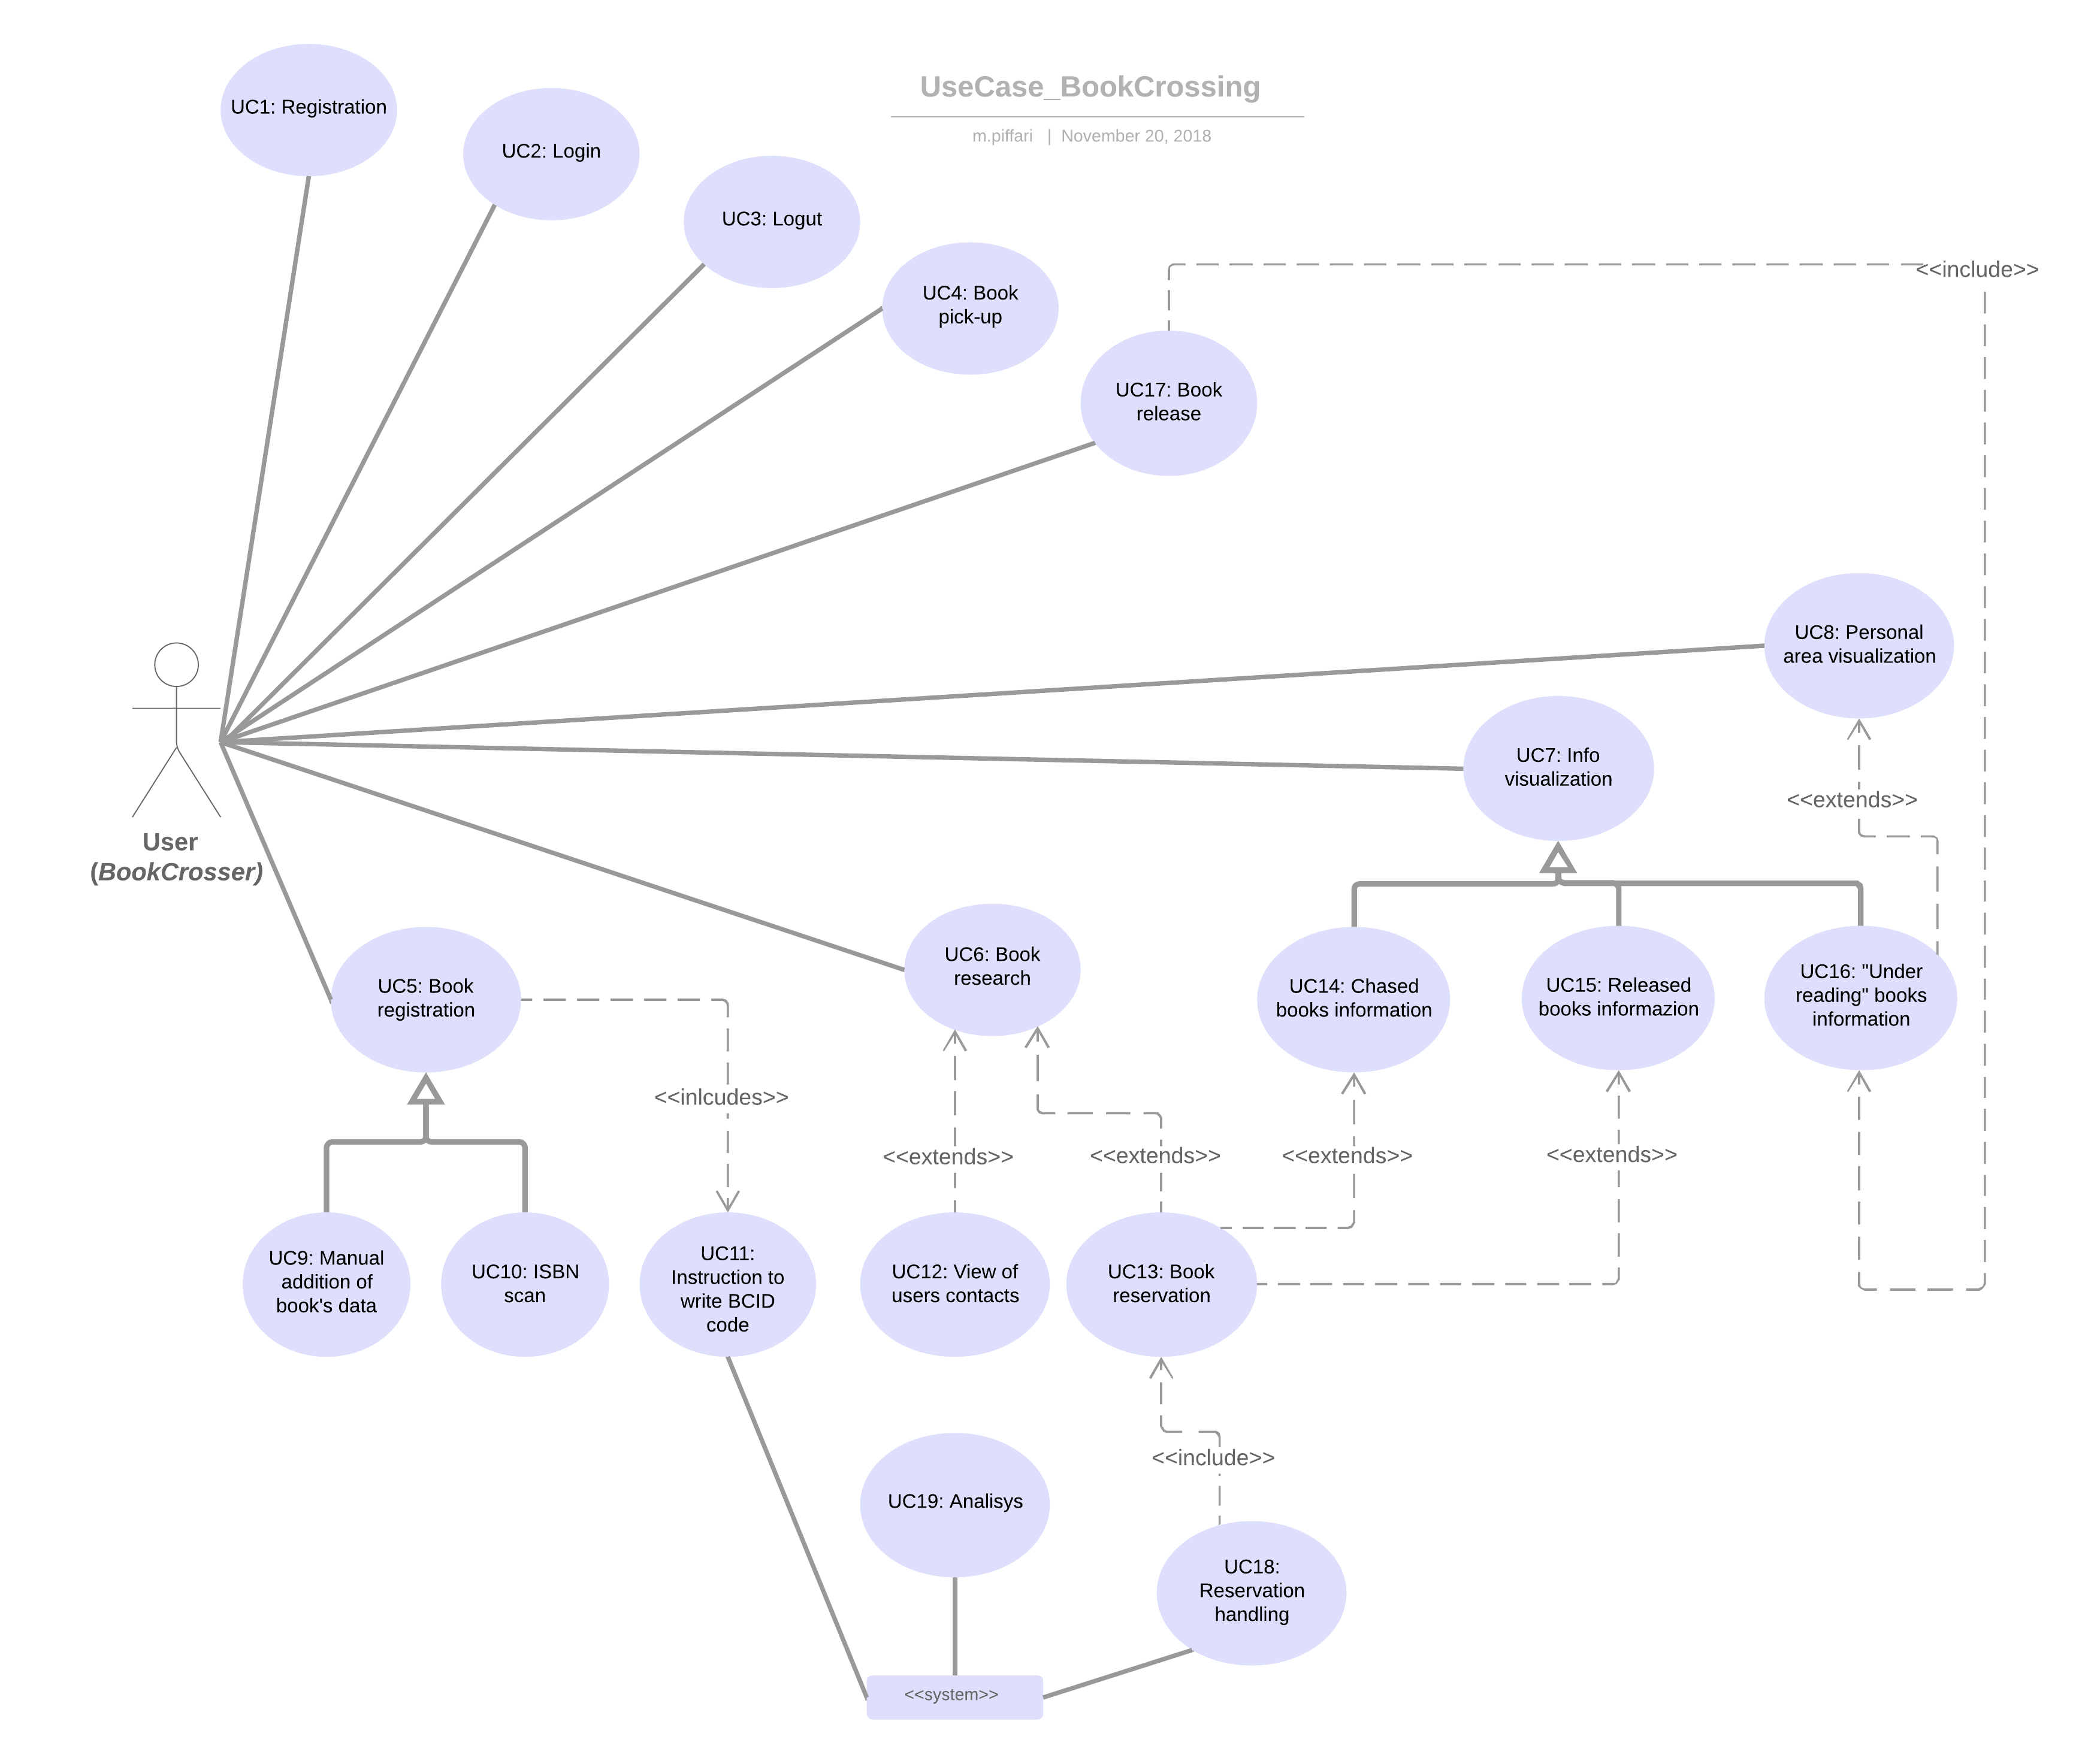
\includegraphics[width=\textwidth]{Immagini/UseCase_BookCrossing}
	\caption{Use cases diagram}
	\label{fig:UsecasesDiagram}
\end{figure}
\newpage
\section{Funzionalità richieste}
\begin{table}[h]
\caption{Panoramica requisiti funzionali progettuali}
\label{tab:Req_utente}
\begin{tabular}{|c|c|c|c|c|c|c}
	\begin{tabular}{p{3cm}|c|c|c|c|c}
		\hline\hline
		\textbf{Nome requisito} & \textbf{ID requisito} & \textbf{Tipologia} & \textbf{Priorità} & \textbf{Requisiti padre} & \textbf{Requisiti figli} \\
		\hline\hline
		Raccolta libro & UR1 & funzionale & alta & & UR2\\
		\hline
		Login utente & UR2 & funzionale & alta & UR1 & UR3, UR4\\
		\hline
		Registrazione utente & UR3 & funzionale & alta & UR2 & \\
		\hline
		Aggiunta libro & UR4 & funzionale & alta & UR2 & UR7, UR9 \\
		\hline
		Ricerca libro & UR5 & funzionale & media & UR2 & UR10 \\
		\hline
		Prenotazione libro & UR6 & funzionale & bassa & UR2 &\\
		\hline
		Visualizzazione info libri chased & UR7 & funzionale & bassa & UR2 &\\
		\hline
		Visualizzazione info libri released & UR8 & funzionale & bassa & UR2, UR4 &\\
		\hline
		Rilascio libro & UR9 & funzionale & alta & UR2, UR4 &\\
		\hline
		Visualizzazione contatti utenti & UR10 & funzionale & bassa & UR2, UR5 &\\
		\hline
		Visualizzazione profilo personale  & UR11 & funzionale & media & UR2 &\\
		\hline
	\end{tabular}
\end{tabular}
\end{table}

\begin{table}[h]
	\caption{Descrizione requisiti non funzionali progettuali}
	\label{tab:Req_utente_descrizione}
	\centering
	\begin{tabular}{|p{5cm}|c|p{5cm}|}
		\hline\hline
		\textbf{Nome requisito} & \textbf{ID requisito} & \textbf{Descrizione} \\
		\hline\hline
		Controllo geolocalizzazione & UR12 & Requisito non funzionalità che permette di verificare che la posizione GPS
		salvata del libro corrisponda, con margine d'accettazione, alla posizione 
		in cui si trova l'utente nel momento in cui vuole raccogliere
		un libro trovato "on the go".\\
		\hline
	\end{tabular}
\end{table}
\section{Stati del libro}
La starup si impone l'obbiettivo di andare a gestire lo scambio di libri all'interno della rete di book-crossing: come visto all'interno dei diversi use-cases, ogni libro nel corso della propria vita all'interno della community, passa di mano in mano attraversando diverse zone.
A questo movimento fisico corrisponde anche un continuo cambio di stato da parte del libro stesso: possiamo riassumere con una \textit{"Finite State Machine"} il percorso che un generico libro segue durante la sua vita.

Riassumendo gli stati di un libro, possono essere:
\begin{itemize}
	\item Out of the network
	\item Available
	\item Under reading
	\item Released
	\item Reserved
	\item Traveling
\end{itemize}

\begin{figure}[h!]
	\centering
	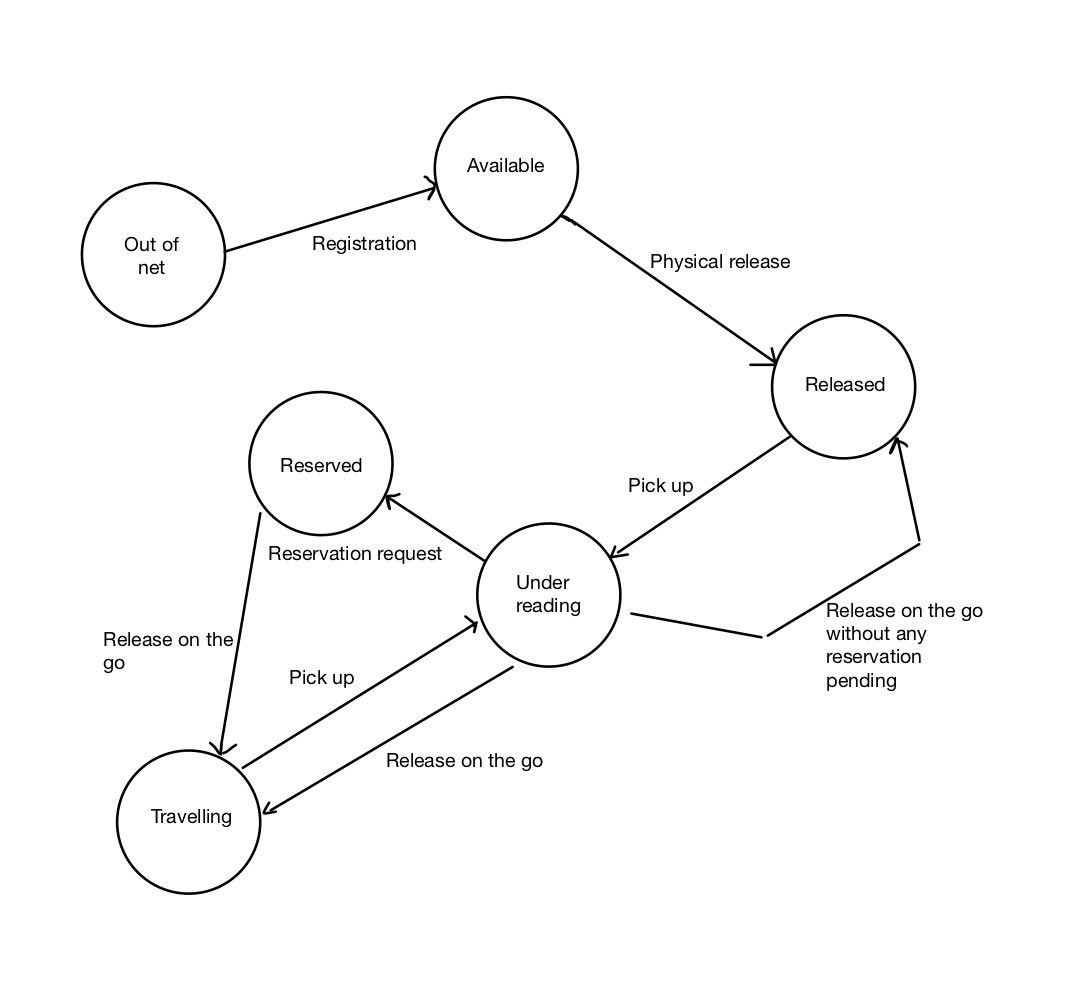
\includegraphics[width=0.6\textwidth]{Immagini/BookState.jpg}
	\caption{Stati del libro all'interno della community}
	\label{fig:BookState}
\end{figure}
\section{Tool chain}
Per la realizzazione del software presentato in questo report sono stati utilizzati i seguenti tool:
\begin{itemize}
	\item \textbf{Modellazione}
	\begin{itemize}
		\item \textbf{Use case diagram}: realizzato con il tool online \textit{Lucid Chart} (\href{https://www.lucidchart.com}{https://www.lucidchart.com});
		\item \textbf{Database architecture}: realizzato con \textit{Vertabelo} (\href{https://www.vertabelo.com/}{https://www.vertabelo.com/});
		\item \textbf{Class diagram - deployment diagram - logical view}: EDrawMax (\href{https://www.edrawsoft.com/en/edraw-max/}{https://www.edrawsoft.com/en/edraw-max/}) e Visual Paradigm (\href{https://www.visual-paradigm.com/}{https://www.visual-paradigm.com/})
		\item \textbf{DB Administration}: Oracle SQL Developer (\href{https://www.oracle.com/it/database/technologies/appdev/sql-developer.html}{https://www.oracle.com/it/database/technologies/appdev/sql-developer.html}).
	\end{itemize}
	\item \textbf{Implementazione software}
	\begin{itemize}
		\item \textbf{Eclipse}: per quanto riguarda l'implementazione del codice Java lato server.
		\item \textbf{Android Studio}: ambiente di sviluppo utilizzato per lo sviluppo della parte mobile.
	\end{itemize}
	
	\item \textbf{Analisi del software}
	\begin{itemize}
		\item \textbf{Espresso - JUnit} per l'analisi dinamica del codice
		\item \textbf{CodeCover - SpotBugs} per l'analisi statica
	\end{itemize}
	\item \textbf{Tool vari}
	\begin{itemize}
		\item \textbf{Versioning}: repository Github gestito tramite interfaccia grafica;
		\item \textbf{Documentazione}: \LaTeX  tramite interfaccia grafica TeXstudio.
		\item \textbf{Canale di comunicazione}: Slack (\href{https://slack.com/intl/en-it/?eu\_nc=1}{https://slack.com/intl/en-it/?eu\_nc=1}).
	\end{itemize}
\end{itemize}

\chapter{Architettura}
\section{Deployment diagram}
\begin{figure}[h]
	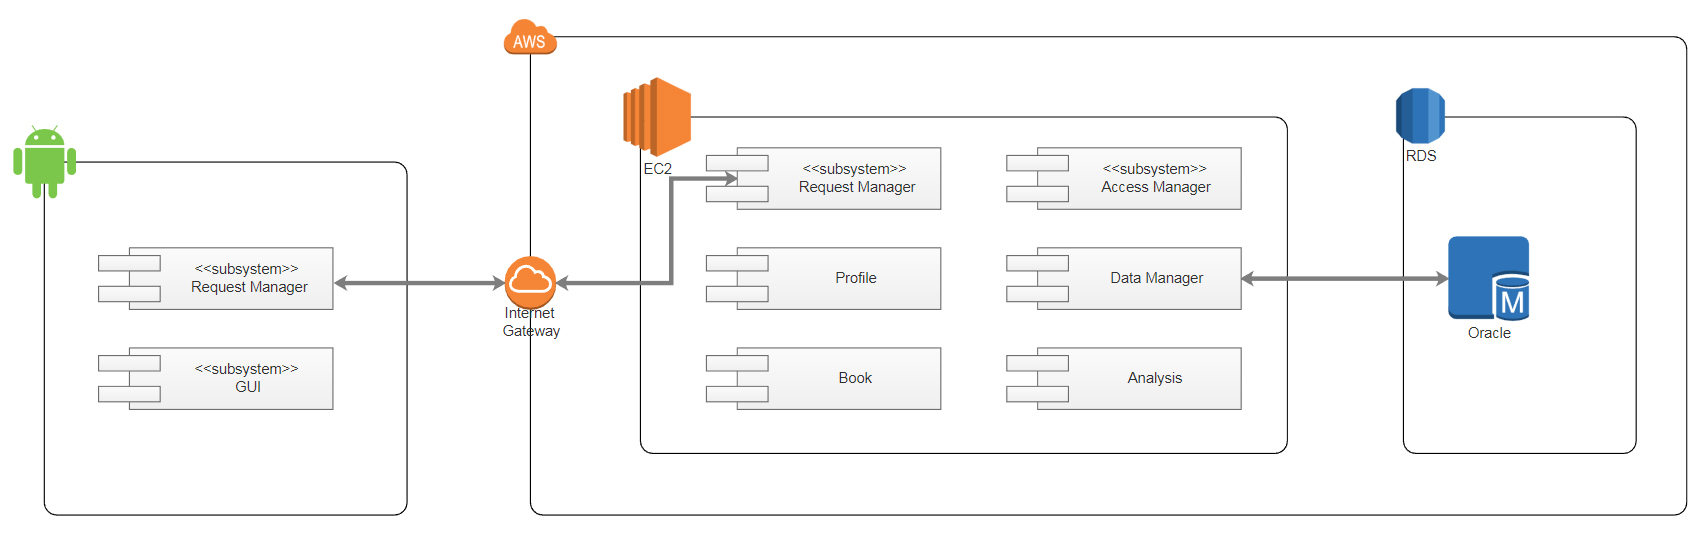
\includegraphics[width=\textwidth]{Immagini/Deployment_Diagram}
	\caption{Deployment Diagram}
	\label{fig:Deployment Diagram}
\end{figure}
\section{Architecture Envisioning}

\begin{figure}[h]
	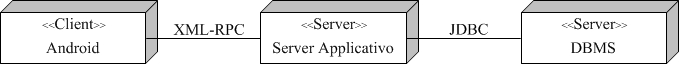
\includegraphics[width=\textwidth]{Immagini/Architecture_Envisoring}
	\caption{Architecture Envisioning}
	\label{fig:ArchitectureEnvisoring}
\end{figure}
\noindent
In figura ~\ref{fig:Deployment Diagram} e ~\ref{fig:ArchitectureEnvisoring} sono mostrati il Deployment Diagram e l'Architecture Envisioning del sistema progettato per lo sviluppo dell’applicazione di Book Crossing. Si può osservare che si tratta di un’architettura \textbf{\textit{Three Tiers}}:
\begin{enumerate}
	\item A sinistra si individua il client, ovvero il dispositivo Android con il quale è possibile interfacciarsi. Al suo interno quindi si può osservare la presenza di un componente relativo all’interfaccia grafica e uno relativo alla gestione delle richieste per invio e ricezione di dati con il server;
	\item Nella parte centrale individuiamo gli altri due layer dell’architettura: server EC2 e Database Relazionale RDS. il fatto di utilizzare Amazon Web Services (AWS) consente di avere questi due elementi a bordo di un unico strato.
\end{enumerate}
\noindent
Per la comunicazione tra smartphone e EC2 utilizziamo un connettore basato su una socket TCP, mentre il server applicativo (EC2) si connette al DBMS (RDS Oracle) tramite il connettore OJDBC (Oracle Java DataBase Connectivity). 
\section{Database architecture}
\begin{center}
\begin{sideways}%[htbp]
	\begin{minipage}{1.3\textwidth}
		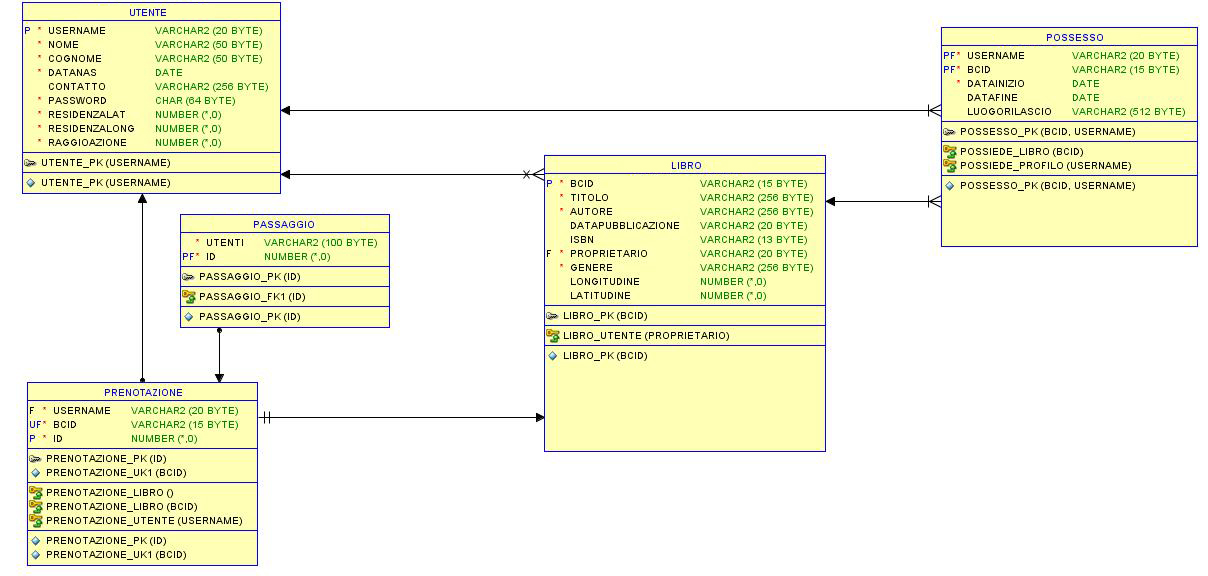
\includegraphics[width=\linewidth,keepaspectratio]{Immagini/db_schema.jpg}
		\captionof{figure}{Modello del databse}
		\vspace{0.2cm}
		\label{fig:xx}
	\end{minipage}
\end{sideways}
\end{center}

La figura 3.3 rappresenta il modello logico del database, le cui entità sono:
\begin{itemize}
	\item \textbf{Utente} : contiene tutti i dati relativi all'utenza registata, ogni utente è identificato da uno \textit{username} univoco;
	\item \textbf{Libro} : contiene tutti i libri presenti nel sistema, ognuno dei quali è identificato da un BCID generato univocamente;
	\item \textbf{Prenotazione} : rappreseta la relazione N:N tra Utente e Libro;
	\item \textbf{Passaggio} : contiene la sequenza di utenti che dovrebbero partecipare in maniera attiva alla prenotazione indicata dalla PK della tabella stessa;
	\item \textbf{Possesso} : questa tabella rappresenta i libri attualmente in possesso dagli utenti iscritti alla community.
\end{itemize}



\part{Iterazione 1}
\chapter{Architettura}
\section{Architettura software}
\begin{figure}[h]
	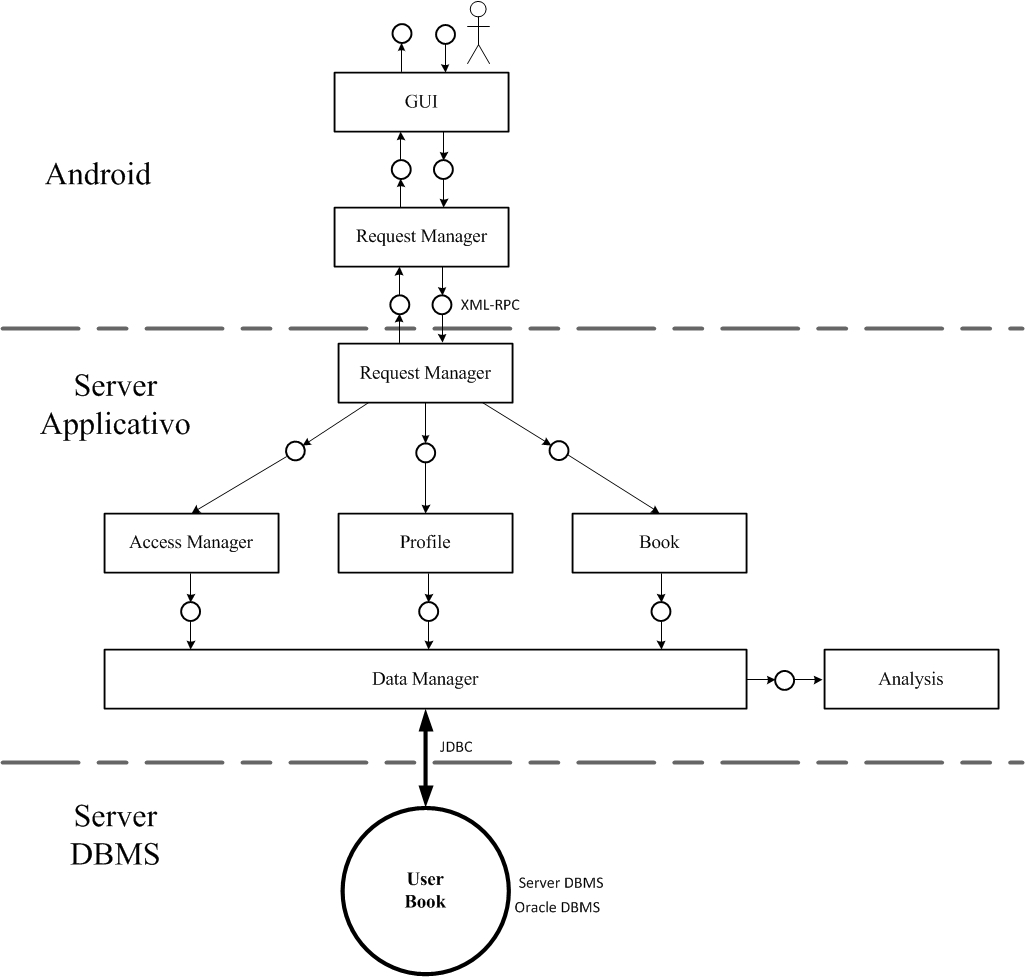
\includegraphics[width=\textwidth]{Immagini/Architettura_Software}
	\caption{Architettura Software}
	\label{fig:ArchitetturaSoftware}
\end{figure}
\newpage
Nella figura ~\ref{fig:ArchitetturaSoftware} è mostrata l'architettura software modellizzata attraverso una rete di Petri. Innanzitutto si può già osservare chè è stata definita seguendo il modello architetturale MVC:
\begin{itemize}
	\item A monte è prevista una parte riservata all'interfaccia grafica, attraverso la quale sarà possibile inviare e ricevere informazioni dal server applicativo. Si vede, infatti, che è prevista una comunicazione bidirezionale tra dispositivo Android e Server.
	\item Al centro sono rappresentate tutte le richieste a cui è in grado di rispondere. Queste, quindi, saranno funzioni implementate lato Server.
	\item Infine, è prevista una banca dati persistente, in questo caso un database relazione, al quale il Server Applicativo accede sia per operazioni di lettura che di scrittura, sempre con lo scopo di far fronte alle richieste provenienti a monte.
\end{itemize}
Si può quindi constatare che non si trattano di strati tra loro indipendenti, poichè il flusso dei dati li coinvolge tutti.
\section{Logical view}
\begin{figure}[h!]
	\centering
	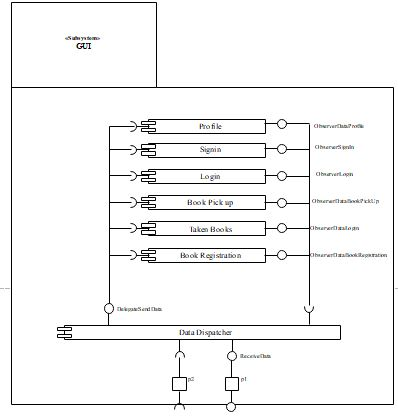
\includegraphics[width=0.8\textwidth]{Immagini/GUI_subsys}
	\caption{Logical view - GUI subsystem}
	\label{fig:LogicalView_GUIsubsys}
\end{figure}
\begin{figure}[h!]
	\centering
	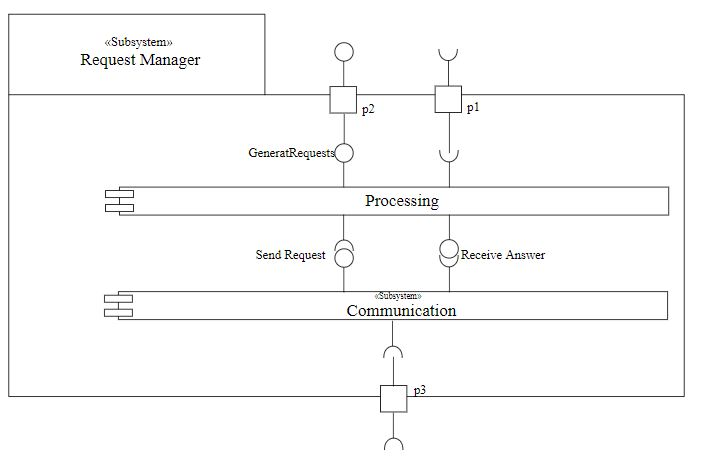
\includegraphics[width=0.8\textwidth]{Immagini/RequestManagerClient_subsys.JPG}
	\caption{Logical view - Request Manager subsystem client side}
	\label{fig:LogicalView_RMsubsys}
\end{figure}
\begin{figure}[h!]
	\centering
	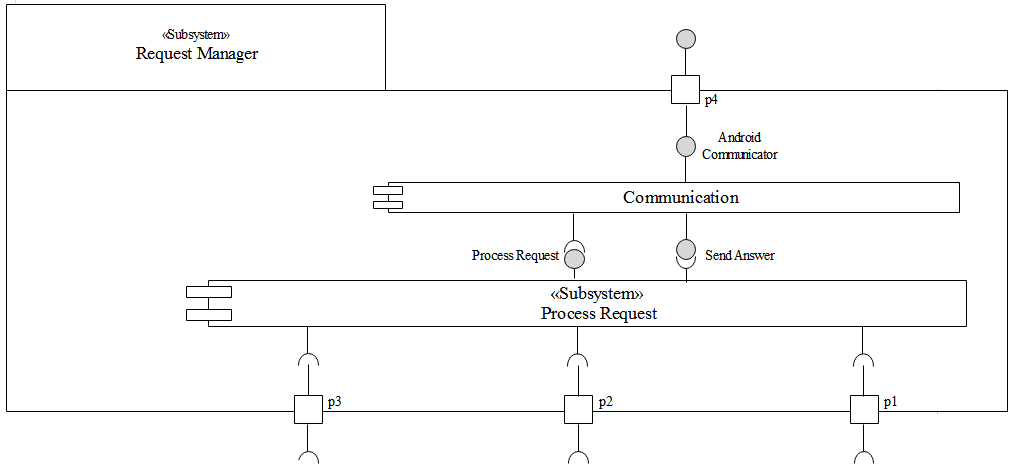
\includegraphics[width=0.8\textwidth]{Immagini/RequestManagerSrv_subsys}
	\caption{Logical view - Request Manager subsystem server side}
	\label{fig:LogicalView_RM_server_subsys}
\end{figure}
\begin{figure}[h!]
	\centering
	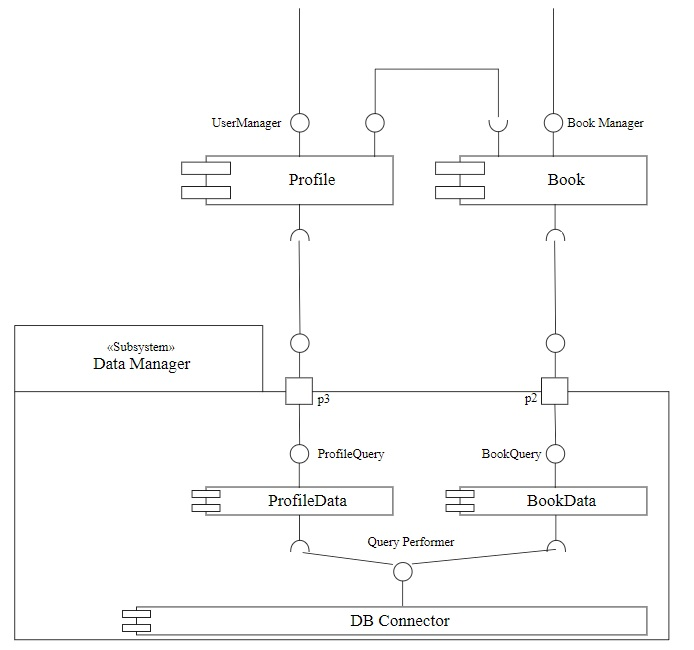
\includegraphics[width=0.8\textwidth]{Immagini/Server_subsys}
	\caption{Logical view - Server functionality}
	\label{fig:LogicalView_ServerSubsys}
\end{figure}
\noindent
Nelle figure ~\ref{fig:LogicalView_GUIsubsys}, ~\ref{fig:LogicalView_RMsubsys}, ~\ref{fig:LogicalView_RM_server_subsys} e ~\ref{fig:LogicalView_ServerSubsys} è mostrata in dettaglio la Logical View del sistema progettato. Si può osservare che segue il modello definito attraverso il pattern archietteturale Model View Controller, dal momento che vengono individuati tre strati, ciascuno dei quali con le seguenti caratteristiche:
\begin{itemize}
	\item\label{subsysGUI} \textbf{Subsystem \textit{"GUI”:}} rappresenta l’interfaccia grafica con la quale l’applicazione si presenterà. Ciascun componente fa riferimento ad ogni view che l'applicazione può mnostrare, e che quindi corrisponde a diffenti casi d'uso dell'applicativo stesso, come l’accesso alla rete di Book Crossing (Login) o registrazione di un  libro.
	
	Questi componenti saranno quindi ovviamente allocati direttamente sul dispositivo mobile: ogni singolo component (\textit{fragment}) avrà legato ad esso, in maniera intrinseca, anche un file \textit{.xml}, il quale permette di definirne l'interfaccia grafica, ovvero come sono posizionati gli elementi visivi.
	
	TODO: spiegazione sintetica delle funzionalità di ogni singolo fragment
	
	\item\label{subsysRequestManager} \textbf{Subsystem \textit{"Request Manager”:}} ha il compito di gestire le richieste provenienti da ciascun componente descritto nel subsystem \textit{GUI”}. Al suo interno sono indicati i componenti attraverso i quali si risponde alle richieste provenienti dal dispositivo mobile.
	
	Una parte di questo \textit{manager} sarà disposta a bordo del dispositivo, permettendo una preelaborazione e assemblamento delle richieste; questo subsystem avrà però anche un implementazione \textit{server side}, che gli permetterà di ricevere tali richieste, rieditarla, secondo quello che è la necessità della richiesta, e poi interacciarsi, in un verso o nell'altro, con la parte di persistenza dei dati.
	\item\label{subsysDataManager} \textbf{Subsystem \textit{"Data Manager":}} ”: rappresenta la comunicazione con il Database. Sono quindi indicati i componenti con i quali il sistema si interfaccerà con la banca dati dell’architettura.
\end{itemize}

Si vede quindi come ogni parte dell'archietettura abbia un compito ben definito: la parte relativa al subsystem \textit{GUI (Graphic User Interface)}, si occupa di gestire l'interazione con l'utente ricevendo e/o mostrando i dati forniti e/o richieste dall'utilizzatore stesso; al suo interno quindi non trovermo codice di logica applicativa ma solamente componenti di gestione \textit{UI}. Esso rappresenta quindi la parte di \textit{\textbf{view}}.
Il subsystem \textit{request manager} invece si occupa di controllare il flusso di dati dall'applicazione al server e viceversa; rappresenta quindi la sezione di \textit{\textbf{controller}} dove è contenuta la \textit{low logic} dell'applicazione.
Infine, il terzo ed ultimo componente della struttura MVC, è rappresentato dal subsystem \textit{data manager}, il quale permette di interfacciarsi direttamente con la base di dati, astrendo tutte le operazione di controllo di accesso al database stesso.
Il modello architetturale MVC è stato poi applicato anche successivamente per la progettazione delle componenti previste per ciascun elemento dell'architettura.
\newpage
\chapter{Analisi dei componenti}
Come già presentato in precedenza, per la definizione dei componenti si è deciso di seguire il pattern architetturale MVC. 
Le componenti che si è deciso di sviluppare durante la prima iterazione sono: 
\begin{itemize}
	\item \textbf{Componente \textit{Manual Book registration:}} La componente \textit{Manual Book registration} fa riferimento all’ UC9 (~\ref{itemize:UC9} ) (figlio del caso d'uso più generico UC5 (~\ref{itemize:UC5} ), ovvero alla funzione di aggiunta di un libro alla rete di Book Crossing per via manuale. La componente si presenta nel seguente modo:
	\begin{itemize}
		\item \textit{GUI:} Interfaccia grafica utilizzata per registrare un libro alla rete di Book Crossing. Verranno quindi messe a disposizione una serie di interfaccie grafiche, composte sostanzialmente da campi da compilare, per aggiungere le informazioni relative al proprio libro, ottenendo poi, successivamente alla registrazione, il relativo BCID;
		\item \textit{Model:} Si fa carico di ricevere le informazioni relative al libro e, sfruttando la parte Data, restituisce alla parte GUI il BCID con il quale siglare il libro;
		\item \textit{Data:} Le informazioni relative al libro che si vuole aggiungere sono memorizzate nel Database RDS, associandolo all'utente che attualmente lo possiede. 
	\end{itemize}
	\item \textbf{Componente \textit{Ricerca:}}  La componente \textit{Ricerca} fa riferimento all’ UC6 
	%(~\ref{itemize:UC6})
	, ovvero alla funzione che permette di andare a ricercare un libro all'interno della piattaforma di Book crossing: questa ricerca può avvenire per titolo, per autore, oppure per entrambi. La componente si presenta nel seguente modo:
	\begin{itemize}
		\item \textit{GUI:} Interfaccia grafica composta da due text book in cui andare ad inserire titolo e/o autore. Essendo possibili tre tipologie di ricerca, come specificato in precedenza, non è necessario compilare entrambi i campi (lo è solamente nel caso in cui si è interessati a compiere una ricerca basandosi su entrambi i vincoli);
		\item \textit{Model:} Gli compete la parte relativa allo smistamento delle richiesta, a seconda del fatto che si stia eseguendo una ricerca per titolo, autore o entrambi;
		\item \textit{Data:} Fornisce, se presenti, le informazioni relative al libro oggetto della ricerca.
	\end{itemize}
\end{itemize}
\chapter{Observer-delegate pattern: la nostra implementazione}
L'applicativo, oltre a seguire un design MVC, per la separazione dei componenti, implementa anche un pattern di comunicazione ad eventi, meglio conosciuto come \textit{pattern observer-delegate}. 
In sostanza, ogni componente che necessita di una certa tipologia di informazioni, si mette in ascolto, registrandosi ad un "servizio" offerto nel nostro caso dal \textit{DataDispatcherSingleton}, il quale va a salvarsi al suo interno un gruppo di riferimenti (delegati) che dovrà poi andare a notificare nel momento in cui risulteranno essere presenti nuove informazioni a cui gli observers stessi sono interessati.
Come si può ben capire si tratta quindi di un pattern molto vicino alla struttura \textit{Publish-Subscribe}, con il quale si definisce una dipendenza uno a molti fra gli oggetti: in sostanza abbiano un oggetto che viene \textit{osservato} e tanti oggetti che \textit{osservano} i cambiamenti di quest'ultimo, come si può vedere nella struttura generica rappresentata in figura ~\ref{fig:ObserverStructure}:

\begin{figure}[h]
	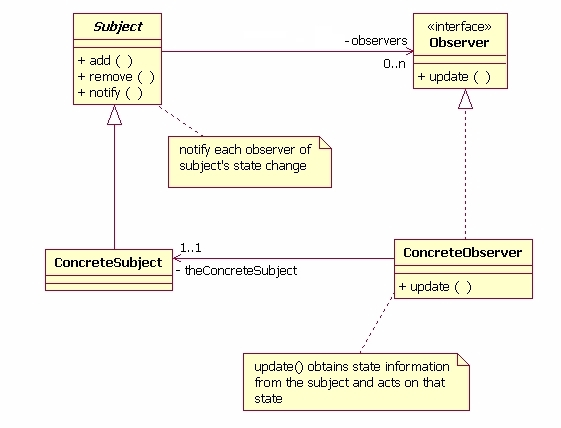
\includegraphics[width=\textwidth]{Immagini/Observer/ObserverTheory.jpg}
	\caption{Struttura generica pattern observer}
	\label{fig:ObserverStructure}
\end{figure}

Questa struttura è stata riprodotta anche nel nostro applicativo, dove possiamo vedere la presenza di alcune struttura caratteristiche di questo pattern: abbiamo una funzionalità di \textit{register}, che, a seconda di quale observer chiama questa funziona, lo pone nel vettore specifico (figura ~\ref{fig:RegisterFunction}). Per evitare di avere dipendenze cicliche, o comunque per mantenere una certa pulizia nei riferimenti tra classi, p necessario che ogni observer, nel momento in cui non necessita più di una certa tipologie di informazioni, vada a deregistrarsi: questa operazione consiste nell'andare a togliere il qualsiasi riferimento all'oggetto in esame dall'interno del \textit{DataDispatcherSingleton}, come fatto in figura ~\ref{fig:UnregisterFunction}.

\begin{figure}[h]
	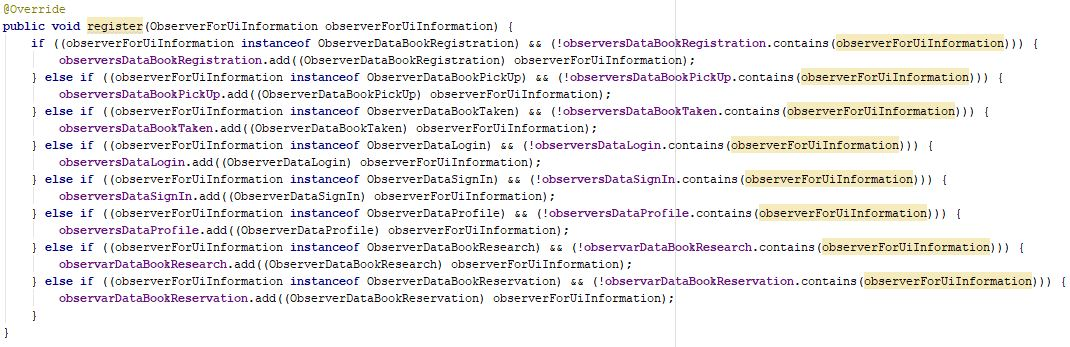
\includegraphics[width=\textwidth]{Immagini/Observer/RegisterToDispatcherData.JPG}
	\caption{Register function}
	\label{fig:RegisterFunction}
\end{figure}

\begin{figure}[h]
	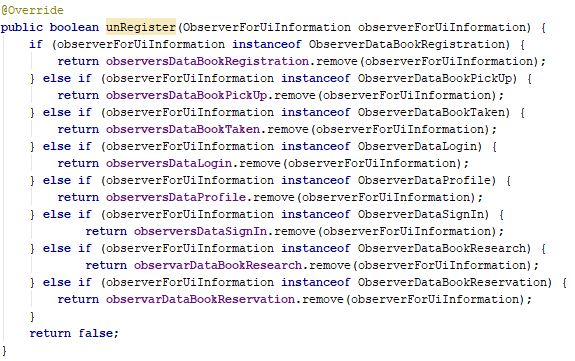
\includegraphics[width=\textwidth]{Immagini/Observer/UnregisterFromDispatcherData.JPG}
	\caption{Unregister function}
	\label{fig:UnregisterFunction}
\end{figure}

Per quanto riguarda invece la parte di \textit{notifica}, abbiamo introdotto un pattern ad eventi custom, che permettesse così di mantenere separata l'implementazione delle informazioni ottenuto da ogni singolo fragment, come si vede nella figura ~\ref{fig:ObserverForUiInformation}.
\begin{figure}[h]
	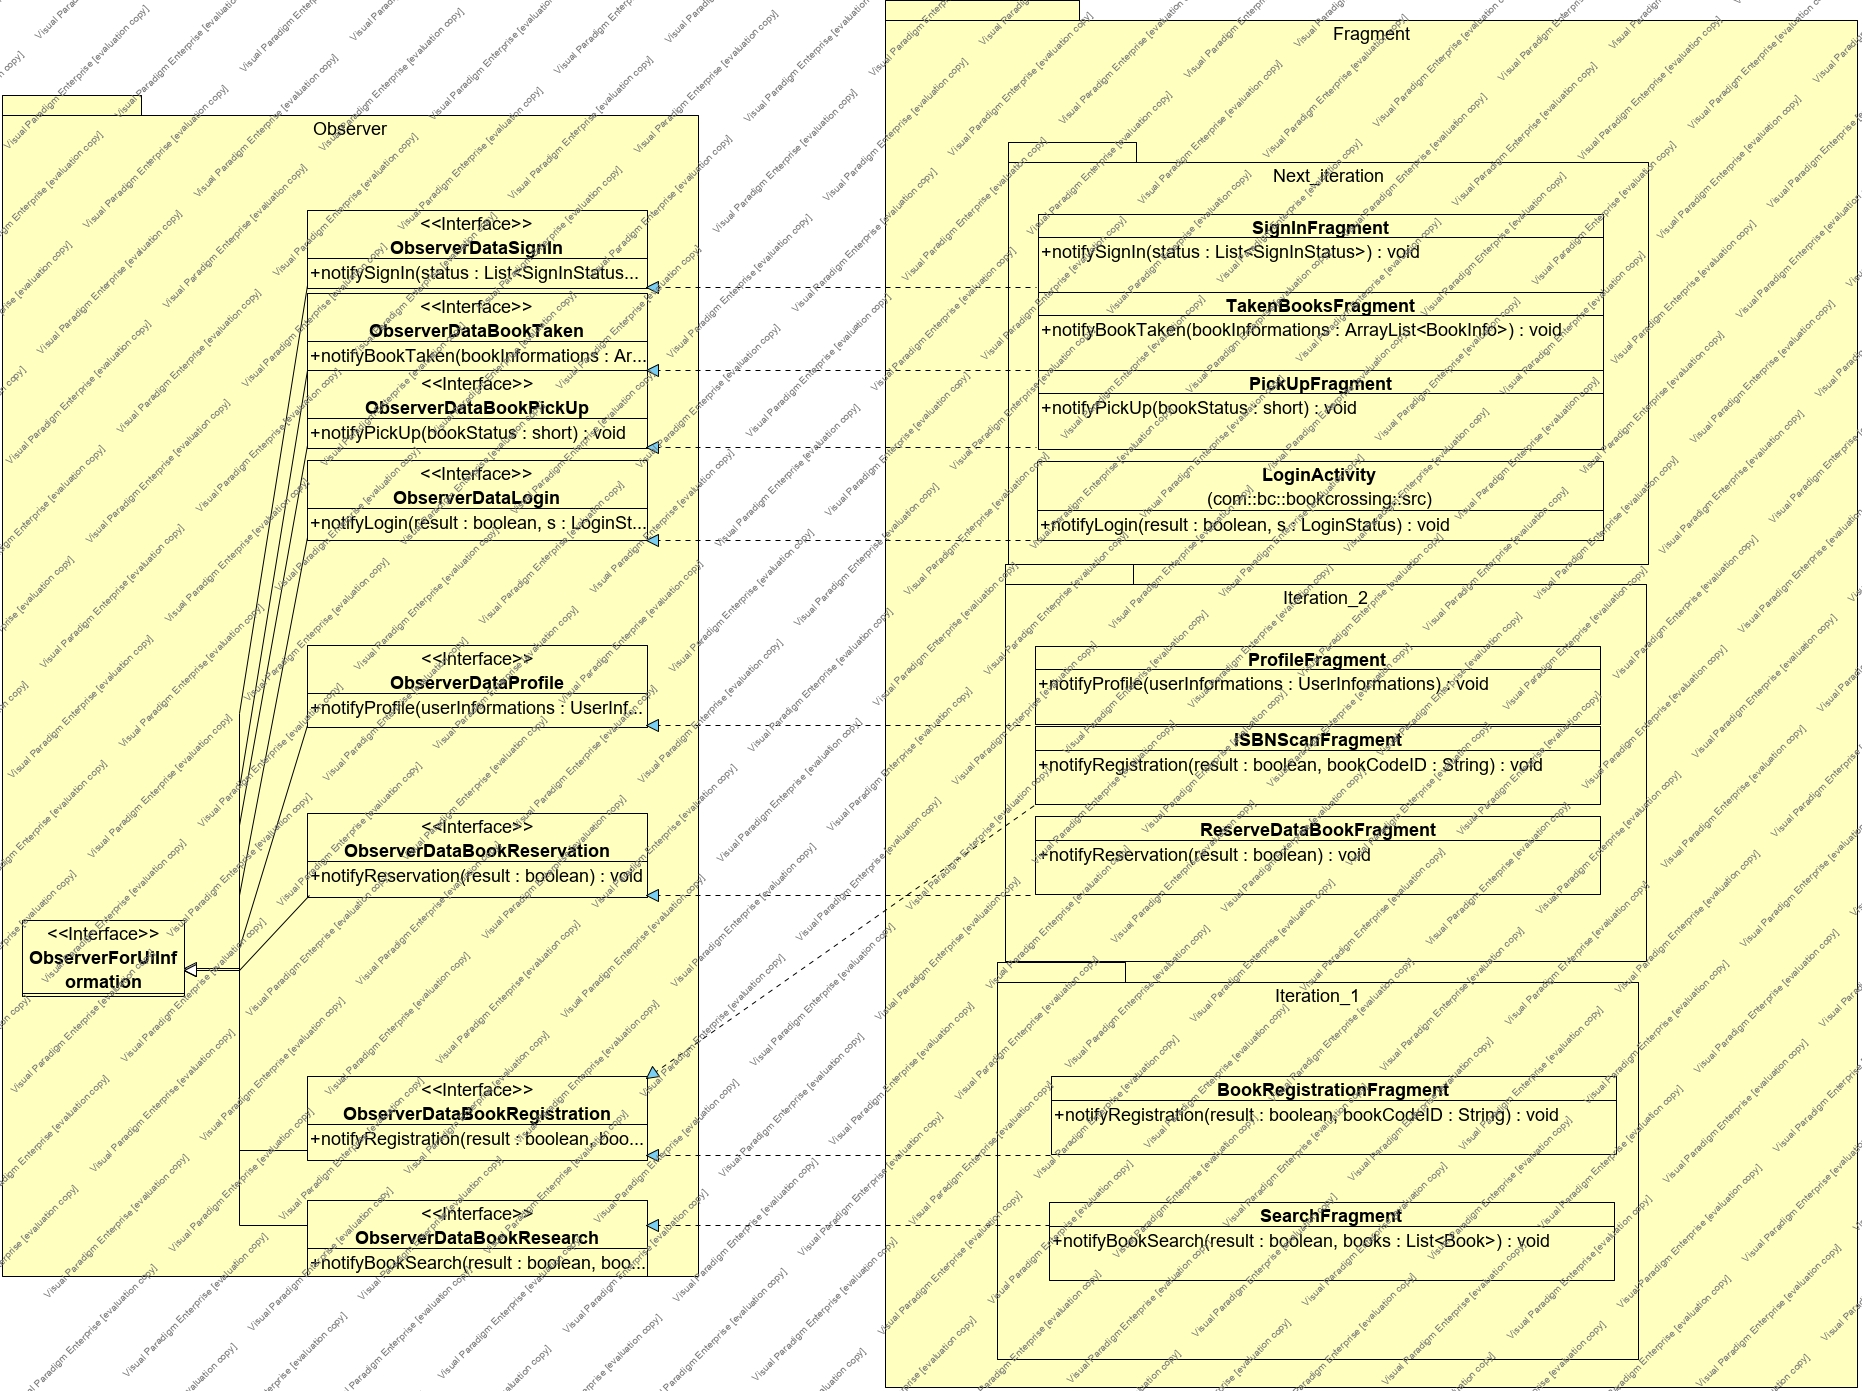
\includegraphics[width=\textwidth]{Immagini/ObserverForUIInformation}
	\caption{Interfaccie per la ricezione degli eventi}
	\label{fig:ObserverForUiInformation}
\end{figure}

Ogni singola interfaccia implementa un'interfaccia comune: questa scelta è stata adotta per rendere del tutto generico il tipo di observer che va a registrarsi per gli eventi forniti dal delegate: infatti, come si può vedere nell'interfaccia \textit{DelegateSendData} (figura ~\ref{fig:DataDispatcher}), chi è interessato ad ottenere informazioni specifiche, si registra come un oggeto di tipo \textit{ObserverForUiInformation}; sarà poi compito del delegate fornire le corrette informazioni, richiamando le corrette funzioni di notifica, le quali sono direttamente implementata all'interno di ogni singola interfaccia concreta.

\begin{figure}[h!]
	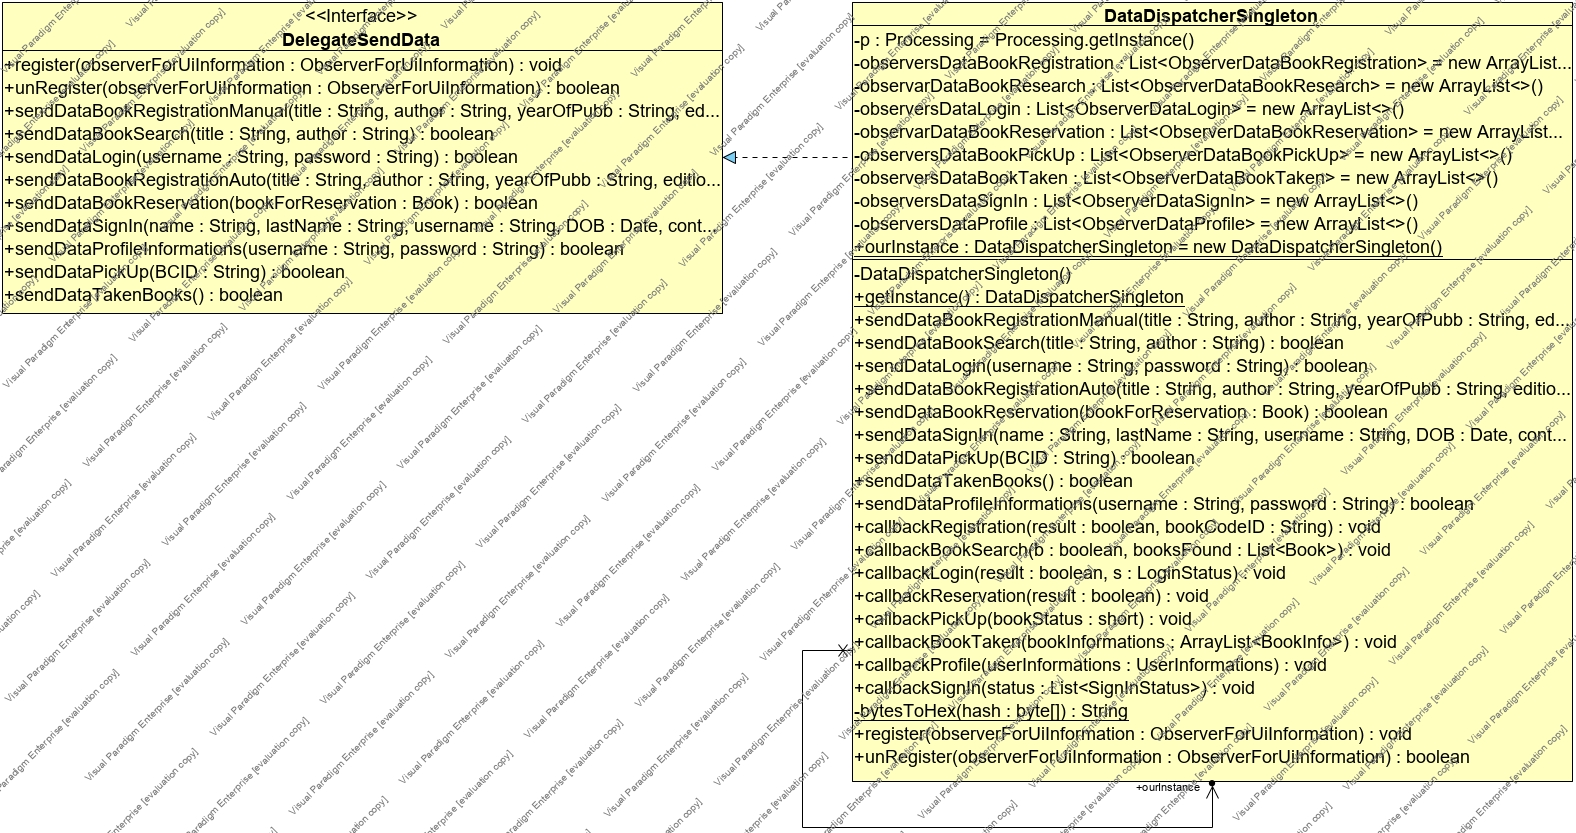
\includegraphics[width=\textwidth]{Immagini/ClassDiagramDispatcherDelegate}
	\caption{Struttura del componente \textit{DataDispatcher}}
	\label{fig:DataDispatcher}
\end{figure}

Si può quindi vedere che, nella struttura predisposta, il \textit{DataDispatcher} lavora come se fosse un \textbf{repository}, ovvero un contenitore di informazioni, che fornisce a tutti gli elementi che si registrano e che ne richiedono la ricezione.

Questi elementi, allo stadio implementativo attuale, sono rappresentati da tutti i fragment, che necessitano di ricevere/inviare informazioni per soddisfare l'interazione con l'utente: come si può notare nelle figure ~\ref{fig:LoginFragment}-~\ref{fig:LoginFragment}-~\ref{fig:BookRegistrationFragment}-~\ref{fig:PickUpFragment}-~\ref{fig:ProfileFragment}-~\ref{fig:SignInFragment}-~\ref{fig:TakenBooksFragment}, ogni singolo fragment è predisposto per ricevere le informazioni di cui ha bisogno, tramite la chiamata delle callback da parte del dispatcher stesso.


\begin{figure}[h!]
	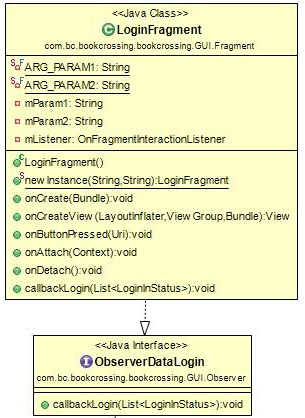
\includegraphics[width=0.5\textwidth]{Immagini/LoginFragment}
	\caption{Struttura del componente \textit{LoginFragment}}
	\label{fig:LoginFragment}
\end{figure}


\begin{figure}[h!]
	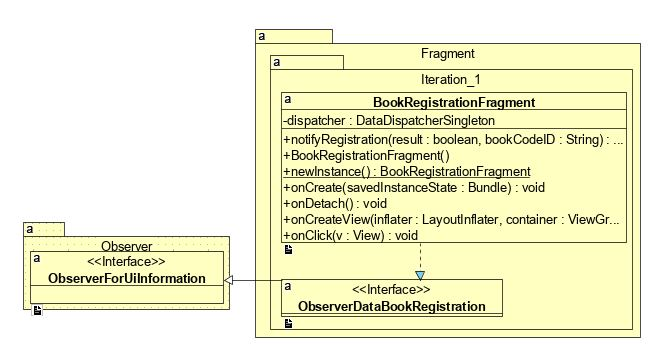
\includegraphics[width=0.5\textwidth]{Immagini/BookRegistrationFragment}
	\caption{Struttura del componente \textit{BookRegistrationFragment}}
	\label{fig:BookRegistrationFragment}
\end{figure}

\begin{figure} [h!]
	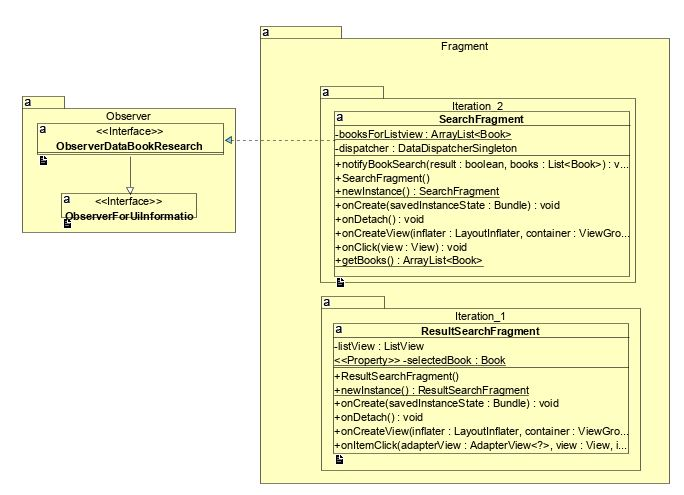
\includegraphics[width=0.5\textwidth]{Immagini/ResearchFragment.jpg}
	\caption{Struttura del componente \textit{ResearchFragment}}
	\label{fig:ResearchFragment}
\end{figure}

\begin{figure} [h!]
	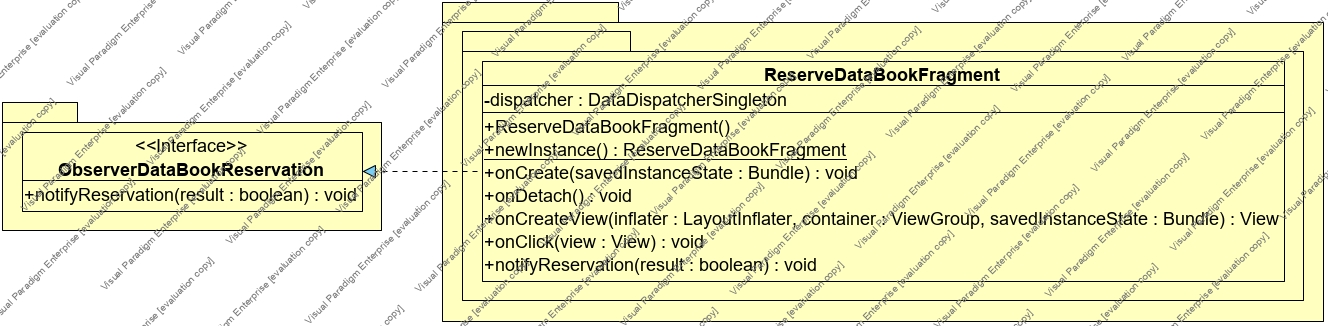
\includegraphics[width=0.5\textwidth]{Immagini/ReservationFragment.jpg}
	\caption{Struttura del componente \textit{ReservationFragment}}
	\label{fig:ReservationFragment}
\end{figure}
\newpage
\chapter{Implementazione comunicazione server}
\section{il framework \textit{Netty}}
Netty è un framework NIO (Non-blocking Input Output) di tipo client-server (i.e. permette una comunicazione asincrona tra client e server di tipo event-driven) che facilita lo sviluppo di applicazioni di rete che utilizzano socket TCP e UDP.

Il framework è disponibile sul Maven Central Repository e può essere scaricato includendo la seguente dependency nel pom.xml del progetto:
\begin{lstlisting} [caption={My Caption},captionpos=b]
<dependencies>
	<dependency>
		<groupId>io.netty</groupId>
		<artifactId>netty-all</artifactId>
		<version>4.1.32.Final</version>
	</dependency>
</dependencies>
\end{lstlisting}

Lato Server creiamo un oggetto singleton di tipo \textit{Communication} il quale inizializza a sua volte un oggetto di tipo \textit{ServerBootstrap} (io.netty.bootstrap.ServerBootstrap).

Quest'ultimo effettua il bootstrap del \textit{ServerChannel}, dove il \textit{ServerChannel} rappresenta il link "primario" (sul port 5000) che accetta ogni connessione di un client e crea un canale "figlio" sul quale avverà tale comunicazione.

\begin{lstlisting} [caption={My Caption},captionpos=b]
private Communication() throws Exception {
	ServerBootstrap b = new ServerBootstrap();

	b.group(bossGroup, workerGroup).channel(NioServerSocketChannel.class).handler(new LoggingHandler(LogLevel.INFO)).childHandler(new ServerInitializer(sslCtx));

	b.bind(PORT).sync().channel().closeFuture().sync();
}
\end{lstlisting}

Al server andiamo ad aggiungere un handler \textit{ServerInitializer} che aggiunge alla pipeline, oltre agli encoder e decoder di default, il \textit{ServerHandler}.

\begin{lstlisting} [caption={My Caption},captionpos=b]
class ServerInitializer extends ChannelInitializer<SocketChannel> {

	private static final StringDecoder DECODER = new StringDecoder();
	private static final StringEncoder ENCODER = new StringEncoder();
	private static final ServerHandler SERVER_HANDLER = new ServerHandler();
	
	@Override
	public void initChannel(SocketChannel ch) throws Exception {
		ChannelPipeline pipeline = ch.pipeline();
		pipeline.addLast(DECODER);
		pipeline.addLast(ENCODER);
		// and then business logic.
		pipeline.addLast(SERVER_HANDLER);
	}
}
\end{lstlisting}

La classe \textit{ServerHandler} è un sottotipo di \textit{SimpleChannelInboundHandler} \\(io.netty.channel.SimpleChannelInboundHandler) il quale fornisce la stringa inviata dal client tramite il metodo seguente.

\begin{lstlisting} [caption={My Caption},captionpos=b]
class ServerHandler extends SimpleChannelInboundHandler<String> {
	
	@Override
	public void channelRead0(ChannelHandlerContext ctx, String request)
				throws Exception {
		int j = request.indexOf(";");
		String username = request.substring(0, j);
		Communication.chcMap.put(username, ctx);
		
		System.out.println("Process request: " + request);
		computeRequest.process(request.substring(j + 1), username);
	}
}
\end{lstlisting}

l'attento lettore avrà notato che il metodo precedente memorizza la coppia (username, channelHandlerContext) all'interno dell'oggetto chcMap di \textit{Communication}, il quale è di tipo HashMap<String, ChannelHandlerContext>, tale informazione è fondamentale al fine di rispondere al clinet tramite canale "figlio" ad esso dedicato e chiuderlo al termine della comunicazione; il metodo invoca l'elaborazione del messaggio ricevuto tramite l'interfaccia \textit{ProcessRequest} (la semantica della stringa request verrà discussa nel paragrafo successivo).


Infine, ma non per importanza, discutiamo l'implementazione dell'interfaccia \textit{SendAnswer} da parte della classe \textit{Communication}:
\begin{lstlisting}
public final class Communication implements SendAnswer{
	~
	public void send(final String username, final String msg) {
		~
		ChannelFuture oo = chcMap.get(username).writeAndFlush(msg + "\r\n");
		
		oo.addListener(new ChannelFutureListener() {
		
			public void operationComplete(ChannelFuture future)	
							throws Exception {
				int count = 0;
				boolean isError = false;
				
				while(!future.isSuccess()) {
					chcMap.get(username).writeAndFlush(msg + "\r\n");
					System.out.println("Retry send response!");
					if(count == 3) {
						isError = true;
						break;
					} else 
						count ++;
				}
				
				~
				
				future.addListener(ChannelFutureListener.CLOSE);
				chcMap.remove(username);
			}
		});
	}
	~
}
\end{lstlisting}
il metodo send si occupa di inviare la risposta relativa alla richiesta ricevuta e nel caso di fallimento ripeterà l'invio fino a un limite di 3 tentativi.
\begin{figure}[h]
	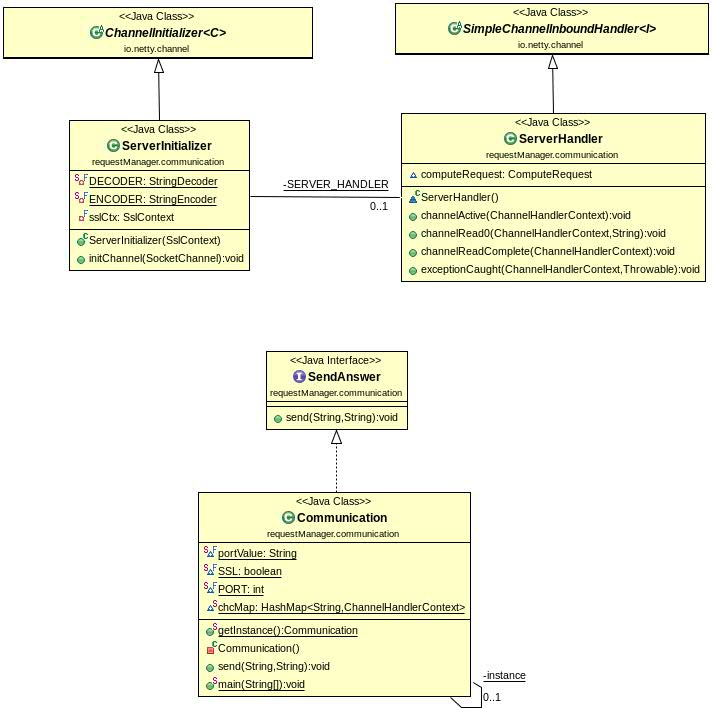
\includegraphics[width=\textwidth]{Immagini/CommunicationPackageServer}
	\caption{Struttura del package \textit{requestManager.Communication}}
	\label{fig:xx}
\end{figure}
\newpage
Lato Client creiamo un singleton \textit{Communication} che implementa il seguente metodo dell'interfaccia \textit{SendRequest} aprendo la connessione con il Server sulla socket (35.180.103.132,5000) e inviando il messaggio al server:
\begin{lstlisting}
public class Communication implements SendRequest {
	private static final String IP = "35.180.103.132";
	public static final String HOST = System.getProperty("host", IP);
	public static final int PORT = 5000;
	~
	@Override
	public boolean send(String data) {
		~
		Bootstrap b = new Bootstrap();
		b.group(group).channel(NioSocketChannel.class).handler(new
					 ClientInitializer(sslCtx));
		ChannelFuture ch = null;
		~
		ch = b.connect(HOST, PORT);
		~
		ChannelFuture lastWriteFuture = null;
		lastWriteFuture = ch.channel().writeAndFlush(data + "\r\n");
		
		//Wait until all messages are flushed before closing the channel
		if (lastWriteFuture != null) {
			~
			lastWriteFuture.sync();
			~
		}		
	}
	~
}
\end{lstlisting}
Tralasciamo la discussione dell'implementazione della classe \textit{ClientInitializer} in quanto simile a quella della classe duale; invece approfondamo l'implementazione di \textit{ClientHandler}: 
\begin{lstlisting}
class ClientHandler extends SimpleChannelInboundHandler<String> {
	@Override
	protected void channelRead0(ChannelHandlerContext ctx, String msg) {
		Processing.getInstance().processAnswer(msg);
		Communication.getInstance().group.shutdownGracefully();
	}
	~
}
\end{lstlisting}
di particolare interesse è il metodo channelRead0 ereditato da \textit{SimpleChannelInboundHandler}, tale metodo viene invocato dal framework ogni qual volta il client riceve un messaggio, quest'ultimo viene elaborato dal singleton \textit{Processing} e il canale di comunicazione viene chiuso.
\begin{figure}[h]
	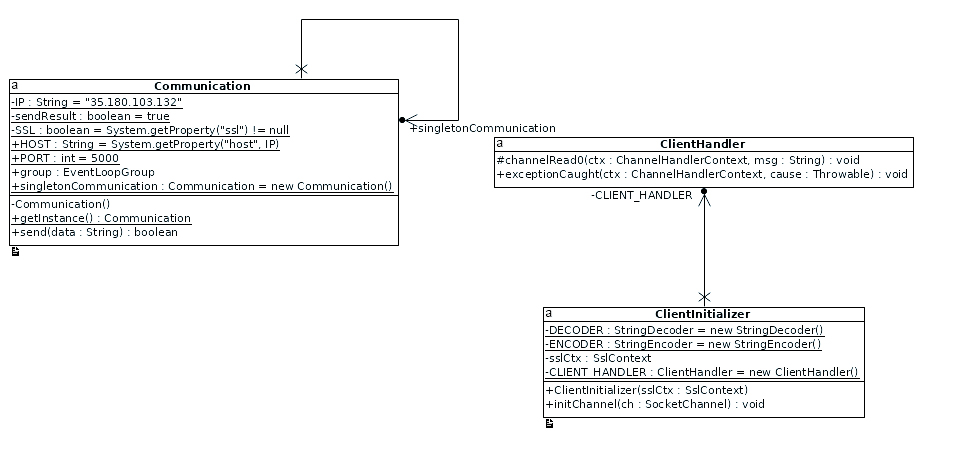
\includegraphics[width=\textwidth]{Immagini/CommunicationPackageClient}
	\caption{Struttura del package \textit{requestManager.Communication}}
	\label{fig:xx}
\end{figure}








\newpage
\section{semantica dei messaggi}
I messaggi inviati dai client sono stringhe che possono essere identificate dalla seguente \textit{RegEx} (\textit{Regular Expression}): 
\begin{center}
	\begin{lstlisting}
	^[a-zA-Z0-9]+;[a-zA-Z0-9]+:[0-9]+;([a-zA-Z0-9]+:[a-zA-Z0-9]+;)+$
	\end{lstlisting}
\end{center}
la cui semantica può essere così rappresentata:
\begin{center}
"<username>;requestType:<tipo>;<richiesta>"
\end{center}
I valori assunti da <tipo> sono i seguenti e corrispondo ai campi definiti all'interno dell'enumerativo \textit{RequestType}.
Durante l'attuale iterazione siamo andati a gestire le richieste relative alle sole due seguenti tipologie di richieste:
\begin{itemize}
	\item 0 -> BOOK\_REGISTRATION\_MANUAL
	\item 8 -> BOOK\_SEARCH
\end{itemize}

Nella seconda iterazione, e nelle successive, è stata pianificata l'implementazione della parte di gestione delle restanti richieste:

\begin{itemize}
	\item 1 -> BOOK\_RESERVATION	
	\item 2 -> LOGIN
	\item 3 -> SIGN\_IN
	\item 4 -> BOOK\_REGISTRATION\_AUTOMATIC
	\item 5 -> PROFILE\_INFO
	\item 6 -> TAKEN\_BOOKS
	\item 7 -> PICK\_UP	
\end{itemize}
La richiesta inviata dal client Android verso il server, ad esempio, per la ricerca di un libro assume la seguente forma:
\begin{center}
	\begin{lstlisting}
	username + ";" + "requestType:" + 0 + ";" + book.encode();
	\end{lstlisting}
\end{center}
\noindent Lato Android, la richiesta vera e propria è preceduta dall'username dell'utente collegato in modo che lato server, qualora, per diversi motivi, l'username fosse invalido, la richiesta venga ignorata a priori.
\\ \noindent
Analogamente possiamo identificare i messaggi inviati dal server come:
\begin{center}
	\begin{lstlisting}
	^[a-zA-Z0-9]+:[0-9]+;([a-zA-Z0-9]+:[a-zA-Z0-9]+;)+$
	\end{lstlisting}
\end{center}
la cui semantica può essere così rappresentata:
\begin{center}
	"requestType:<tipo>;<risultato>"
\end{center}

\noindent Ad esempio, nel caso di invio di una richiesta da parte del server verso lato Android in merito alla registrazione manuale di un libro andata a buon fine, la stringa assume il seguente formato:
\begin{center}
	\begin{lstlisting}
		"requestType:0;result:" + 1 + ";BCID:" + bcid
	\end{lstlisting}
\end{center}
dove \textit{bcid} è il codice alfanumerico generato casualmente dal server per identificare il libro all'interno della rete di Book Crossing.
Qual'ora, invece, il server riceva una richiesta con un tipo errato la risposta del server è la seguente:
\begin{center}
	\begin{lstlisting}
	"requestType:10000;result:KO_RequestType"
	\end{lstlisting}
\end{center}





\newpage
\chapter{Parte algoritmica: \textit{reservation handler}}
La gestione delle prenotazioni dei libri è una delle parte innovative introdotte dalla start up: questo servizio mira a sfruttare la flessibilità della community di sharing, basata sull'ideale di open-source, per comunque offrire un seervizio mirato ed attento alle necessità del lettore.

Ogni utente, purchè sia registrato all'interno del servizio di Book-sharing, può prenotare un determinato libro che si trova nello stato "Under reading".

Andiamo ad evidenziare gli attori coinvolti in questa operazione:
\begin{itemize}
	\item \textbf{\underline{Lettore} [L]:} esso rappresenta l'utente, registrato nella community, che possiede il libro oggetto della prenotazione. Indichiamo con:
	\begin{itemize}
		\item \textbf{{\LARGE $r_{L}$}:} raggio d'azione del lettore;
		\item \textbf{{\LARGE $ z_{0} $}:} zona di residenza (espressa come coordinate puntuali).
	\end{itemize}
	\item \textbf{\underline{Prenotanti} [$ P_{i}$ con $i=1,...,N $]:} rappresentano l'insieme degli utenti, tutti interessati ad uno specifico libro in possesso dell'utente \textbf{L}.
	Nello specifico l'indice \textit{i-esimo} indica l'ordine temporale con cui sono giunte le prenotazioni per lo specifico libro.
	Oltre a questa informazione, ogni utente, rappresentando un generico utente della community, avrà fornito, al momento della registrazione, le seguenti informazioni:
	\begin{itemize}
		\item \textbf{{\LARGE $r^{P}_{i}$} con $i=1,...,N $:} raggio d'azione del lettore;
		\item \textbf{{\LARGE $z^{P}_{i}$} con $i=1,...,N $:} zona di residenza.
	\end{itemize}

	L'algoritmo può essere scomposto in due macro-blocchi:
	\begin{itemize}
		\item \textbf{Step 0:} questo fase viene realizzata nel momento in cui il sistema inizia ad analizzare tutti gli utenti che hanno effettuato una prenotazione per un determinato libro che si trova nello stato di "Under reading".
		
		Tutti gli N prenotanti \textit{$ P_{i} $} vengono ordinati in base alla distanza dal lettore \textit{L}, indipendentemente da quello che è l'ordine temporale con cui è stata effettuata la prenotazione: la quantità di cui si terrà (come si può vedere nella figura ~\ref{fig:DistanceAlgorithm}) conto sarà quindi la distanza
		{\LARGE \begin{equation}
			|z^{p}_{i}-z_{0}|
		\end{equation}}
		\begin{figure}[h!]
		\centering
		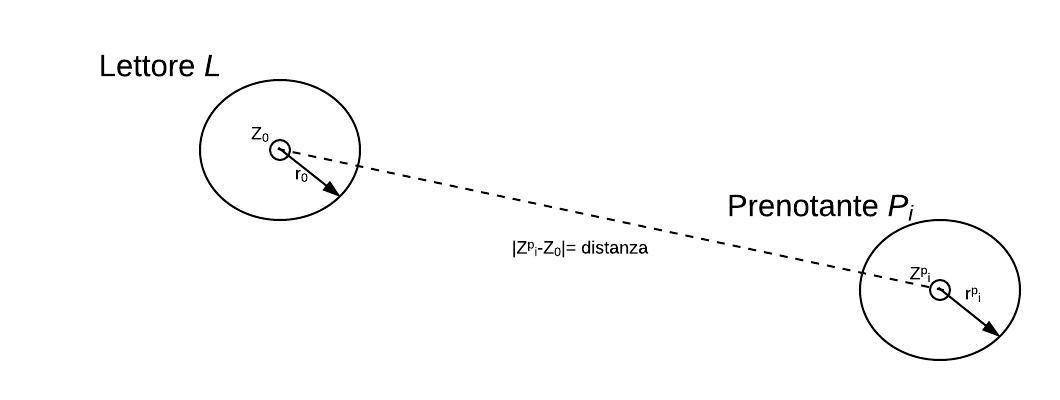
\includegraphics[width=0.8\textwidth]{Immagini/Algoritmo_Explanation}
		\caption{Distanza tra lettore e prenotante i-esimo}
		\label{fig:DistanceAlgorithm}
		\end{figure}
	
		Questo ordinamento corrisponde quindi sostanzialmente a creare una \textit{priority queue} in cui si va ad assegnare una maggiore priorità all'utente la cui zona di residenza è più vicina a quella del lettore in possesso del libro richiesto.
		
		\item \textbf{Step 1:} in questo macro-blocco andiamo effettivamente ad applicare l'algoritmo \textit{smart} per poter soddisfare, nella maniera migliore, le esigenze di ogni utente della community.
		
		
		L'idea di base è che, se lettore e prenotante hanno possibilità di incontrarsi, ovvero se i loro raggi d'azione si sovrappongono, essi potranno accordarsi direttamente sul luogo dello scambio, rendendo \textit{"safety"} il passaggio del libro: questo scambio avverrà ovviamente in una zona all'interno dell'intersezione dei raggi d'azione, come mostrato in figura ~\ref{fig:Zona_incontro}.
		
		\begin{figure}[h!]
			\centering
			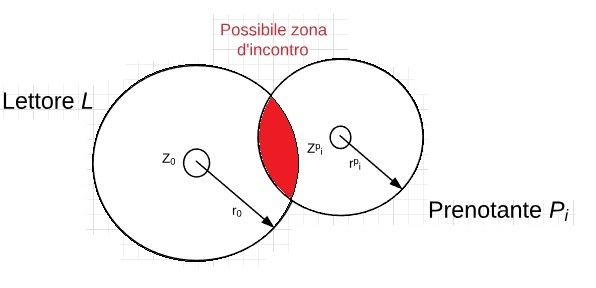
\includegraphics[width=0.6\textwidth]{Immagini/Algorithm_PuntoIncontro.jpg}
			\caption{Zona d'incontro tra lettore e prenotante}
			\label{fig:Zona_incontro}
		\end{figure}
	
		Nel caso in cui invece, i due utenti interessati non abbiano la possibilità di trovare un luogo comune in cui potersi scambiare il libro direttamente, si avrà che, la rete di users appartenenti alla community farà da tramite, per portare il libro \textit{"coast-to-coast"}.
		Quindi, tramite un semplice pseudo-codice, possiamo scrivere il nostro algoritmo come
	
		\begin{algorithm}[H]
			\SetAlgoLined
			\KwData{Users and their informations}
			\KwResult{Optimum path from reader to reserver}
			Step 0 (intilization)\;
			\eIf{Distanza <= 0}{
				Trova un punto d'incontro nell'unione delle delle area;
				
				Notifica gli utenti di dove potersi scambiare direttamente il libro;
			}{
				Crea la rete di utenti che faranno da tramite tra lettore e prenotante;
				
				Ricercare il cammino ottimo (il libro si muoverà \textit{hand-to-hand});
			}
			\caption{Algoritmo di gestione della prenotazione}
		\end{algorithm}
		
		
		Nello specifico il calcolo della distanza avverrà tramite la funzionalità \textit{checkOverlap(Lettore, Prenotante)}, la quale andrà a verificare che:
		
		{\LARGE \begin{equation}
			|z^{p}_{i}-z_{0}|-r_{0}-r_{i}<=0
		\end{equation}}
		
		ovvero che i raggi d'azione si sovrappongano o meno.
		
		Nel caso in cui i due utenti non abbiano possibili punti d'incontro (Distanza $>= 0 $), dobbiamo selezionare gli utenti tramite il quale il libro in questione potrà viaggiare: l'idea base è quindi quella di costruirsi un'area circolare di centro pari alla metà della congiungente del punto $ z_{0} $ (zona di residenza lettore) e $ z^{p}_{i} $ (zona di residenza prenotante).
		Andremo poi a selezionare tutti gli utenti che si trovano all'interno di questa circoscrizione.
		In passi sequenziali, possiamo scrivere:
		
		\begin{algorithm}[H]
			\SetAlgoLined
			\KwData{Zona di residenza e raggio d'azione di utente lettore e prenotante}
			\KwResult{Elenco di utenti attraverso cui il libro dovrà spostarsi \textit{hand-to-hand}}
			
			
			Il raggio della circoscrizione di utenti coinvolti sarà pari alla distanza
			\[ \bar{Z} = \dfrac{1}{2} |z^{p}_{i}-z_{0}| \]
			\For{Tutti gli utwnti $ z_{i}^U $ nella community}{
			\If{$ (Distanza(z_{0},z_{i}^U)) <= \bar{Z} $ oppure $ (Distanza(z_{i}^P,z_{i}^U)) <= \bar{Z} $  }{
				
				Seleziono l'utente $ z_{i}^U $ e lo inserisco nella lista (\textit{HandToHandUsers}) dei possibili utenti che potrebbero partecipare attivamente al prestito;
			}
			}
			Creiamo il collegamento tra gli users della lista \textit{HandToHandUsers} il cui raggio d'azione si sovrappone\;
			\caption{Creazione del percorso tra lettore e prenotante}
		\end{algorithm}
		
		Quindi, alla fine dello step 1, avremo individuato tutti gli utenti i quali potrebbero partecipare attivamente alla realizzazione di un prestito: il risultato ottenuto sarà quindi come quello in figura ~\ref{fig:UsersNet}.
						
		\begin{figure}[h!]
			\centering
			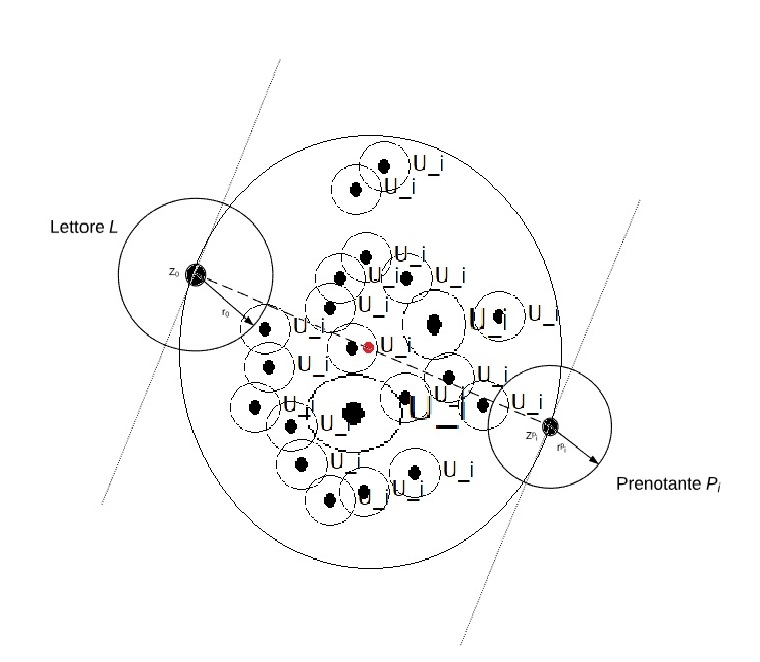
\includegraphics[width=0.8\textwidth]{Immagini/Algorithm_UsersNet}
			\caption{Rete di utenti che potrebbero essere attivi nel prestito}
			\label{fig:UsersNet}
		\end{figure}
		
	\end{itemize}
\end{itemize}

//TODO: move this comment to documentation

// Insieme di candidati: users == overlapping users
// Funzione obbiettivo: minimizzare i km che il libro deve fare / minimizzare il numero di utenti tra cui fare
// il passamano --> la scelgo in maniera epsilon - greedy


// Epsilon for epsilon greedy algorithm: during the path calculation for the reservation
// we choose usually the next user, as the nearest one.
// Using the greedy algorithm, with a probability that depends on the epsilon variable value, we choose the user
// with the biggest radius.
// epsilon lower --> algorithm stronger (always foound path to me)
// epsilon higher --> algorithm found sorthest path
\part{Iterazione 2}
\chapter{Analisi dei componenti}
Le componenti che invece si è deciso di andare a sviluppare durante la seconda iterazione sono: 
\begin{itemize}
	\item \textbf{Componente \textit{Automatic Book registration:}} la componente \textit{Automatic Book registration} fa riferimento all’ UC10
	%(~\ref{itemize:UC10})
	(figlio del caso d'uso più generico UC5 
	%(~\ref{itemize:UC5})
	); questa funzionalità consente di ottenere, in maniera del tutto automatica, le informazioni necessarie per registrare uno specifico libro all'interno della piattaforma di book crossing. La componente si presenta nel seguente modo:
	\begin{itemize}
		\item \textit{GUI:} interfaccia grafica utilizzata per registrare un libro, in maniera automatica, nella rete di Book Crossing. Verranno quindi messe a disposizione una serie di interfaccie grafiche, le quali permetteranno di scansionare il codice ISBN del libro deisderato, unitamente ad una parte GUI utilizzata per mostrare le informazioni relative al libro che è appena stato scansionato.
		\item \textit{Model:} si fa carico di ricevere le informazioni relative al libro e, sfruttando la parte Data, restituisce alla parte GUI il BCID con il quale siglare il libro;
		\item \textit{Data:} le informazioni relative al libro che si vuole aggiungere sono memorizzate nel Database RDS, associandolo all'utente che attualmente lo possiede. 
	\end{itemize}
	\item \textbf{Componente \textit{Login:}}  la componente \textit{Login} fa riferimento all’ UC13 
	%(~\ref{itemize:UC13})
	, ovvero alla funzione che permette ad un utilizzatore dell'applicazione di loggarsi all'interno della piattaforma di Book Crossing, potendo così effettuare operazioni di suo interesse sui testi disponibili.
	La componente si presenta nel seguente modo:
	\begin{itemize}
		\item \textit{GUI:} interfaccia grafica, composta da due caselle di testo, le quali devono essere riempite con username e password, unitamente ad un pulsante che permette di iniviare la richiesta/verifica di login corretto. Per chi non fosse già registrato, è fornita la possibilità di iscriversi alla piattaforma (questo però rappresenta un caso d'uso separato);
		\item \textit{Model:} si fa carico di verificare la coerenza dei dati inseriti tramite il componente grafico, restituendo l'esito a chi ha appena tentato di effettuare il login.
		\item \textit{Data:} le informazioni relative all'utente che sta tentando di loggarsi.
	\end{itemize}
	\item \textbf{Componente \textit{Book reservation:}}  La componente \textit{Book reservation} fa riferimento all’ U13 (~\ref{itemize:UC13} ), ovvero alla funzione di prenotazione di un libro, la quale richiede prima un'operazione di ricerca dello stesso all'interno della community e poi, se possibile, permette di effettuare la prenotazione  effettiva. La componente si presenta nel seguente modo:
	\begin{itemize}
		\item \textit{GUI:} interfaccia grafica utilizzata per poter procedere con la prenotazione di un libro della rete di Book Crossing. In questo caso sarà possibile compiere tale azione attraverso una procedura di ricerca del libro, oppure navigando nella propria sezione personale del profilo;
		\item \textit{Model:} si fa carico di gestire la coda relativa alla prenotazione di un determinato libro, in modo da poterle soddisfare. La gestione e la computazione della prenotazione è affidata ad un algoritmo il quale va ad appoggiarsi alla parte Data per poter risalire ai dati dei richiedenti;
		\item \textit{Data:} le informazioni relative al libro che si vuole prenotare e agli utenti richiedenti le quali sono memorizzate nel Database.
	\end{itemize}
\end{itemize}
Partendo dalla figura \ref{fig:Diagramma della class ComputeRequest} relativa a quanto sviluppato nella precedente iterazione, possiamo andare ad osservare come, nella successiva immagine, il medesimo diagramma delle classi si completa nel seguente modo:
\begin{figure}[h]
	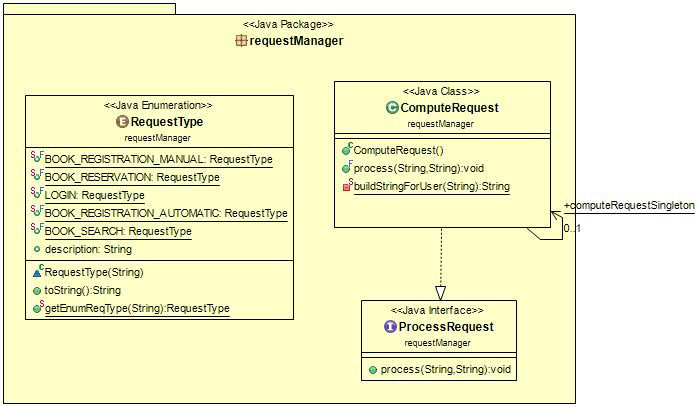
\includegraphics[width=\textwidth]{Immagini/UML_ComputeRequestServer2}
	\caption{Diagramma della classe ComputeRequest}
	\label{fig:Diagramma della class ComputeRequest2}
\end{figure}
\\ \noindent
Si può notare infatti come alla \textbf{\textit{RequestType}} si aggiungano 3 casi in più, relativi proprio ai nuovi componenti sviluppati in questa seconda iterazione. Allo stesso modo anche il codice si completa così
\begin{lstlisting}[caption={Tipologia di richieste aggiuntive gestite durante la seconda iterazione},captionpos=b]
case BOOK_RESERVATION:
	boolean rs = book.reserve(username);
	Communication.getInstance().send(username, "requestType:1;result:" + (rs?1:0));
	break;
case LOGIN:
	Communication.getInstance().send(username, "requestType:2;result:" + "Success" + ";" + buildStringForUser(username));
	break;
case BOOK_REGISTRATION_AUTOMATIC:
	result = b.insert();
	Communication.getInstance().send(username, "requestType:4;result:" + (result?1:0) + ";BCID:" + b.getBCID());
	break;
\end{lstlisting}

Questo si va ad aggiungere a quanto sviluppato nella prima iterazione: a questo punto possiamo quindi gestire le richieste del client compilate nel formato descritto relative ai componenti disponibili nella prima e seconda iterazione.

\end{document}
